%\documentclass[10pt,preprint]{aastex}  % for e-submission to ApJ
%\documentclass[12pt,preprint2]{aastex}  % for e-submission to ApJ - two column
\documentclass[onecolumn]{emulateapj}  % this makes everything look like ApJ

\usepackage{graphicx, natbib, color}

%%%% PUT NEW COMMANDS AND DEFINITIONS HERE %%%%
\input{local-commands}


%%%%%%%%%%%%%%%%%%%%%%%%%%%%%%%%%%%%%%%%%%%%%

% Paper Outline  (last updated June 15, 2009)
%
% 1.  Introduction [GB,MN]
% 2.  Overview [GB]
% - including both equations and a few paragraph overview of how each method works
% - this might have section 2.1, 2.2, etc. corresponding to very brief overviews of section 3.1, 3.2, etc.
% 3.  Numerical methods
%  3.1 AMR [GB]
%  3.2. Hydro: ZEUS [GB]
%  3.3. Hydro: PPM [GB,AK]
%  3.4. Gravity [GB]
%  3.5. Particle Integration [GB]
%  3.6. Chemistry [BWO]
%  3.7. Star formation & Feedback [BWO]
%  3.8. Timestep constraints [BWO,GB]
% 4. Software Implementation
% - maybe this could be split up by into sections 4.1, 4.2, 4.3, etc. using the same scheme as section 3 [same responsibilities as 3]
% 5. Parallelism 
% 5.1. Parallel strategy [GB, RH]
% 5.2. Parallel performance [JB, GB, RH]
% 6. Code Tests [All]
% 7. Summary and Conclusions
%
%%%%%%%%%%%%%%%%%%%%%%%%%%%%%%%%%%%%%%%%%%%%%

\citestyle{aa}  % correct formatting for ApJ style files

\begin{document}

\title{Enzo: An Adaptive Mesh Refinement Code for Astrophysics}
\author{Greg Bryan\altaffilmark{1}, Michael L. Norman\altaffilmark{2}, 
Brian W. O'Shea\altaffilmark{3}, Robert Harkness\altaffilmark{4}, Tom Abel\altaffilmark{5},
David C. Collins,\altaffilmark{2} 
Alexei Kritsuk\altaffilmark{2} and James Bordner\altaffilmark{2} }

\altaffiltext{1}{ Department of Astronomy, Columbia University,
New York, NY, 10027, U.S.A.  Email: gbryan@astro.columbia.edu }
\altaffiltext{2}{Center for Astrophysics and Space Sciences,
University of California at San Diego.
Email: mnorman,dcollins,akritsuk,jbordner@cosmos.ucsd.edu}
\altaffiltext{3}{Theoretical Astrophysics (T-6), Los Alamos National
Laboratories.  Email:  bwoshea@lanl.gov}
\altaffiltext{4}{San Diego Supercomputing Center, University of California
at San Diego.  Email: harkness@sdsc.edu}
\altaffiltext{5}{Kavli Institute for Particle Astrophysics and Cosmology,
 Stanford University.  Email:  tabel@stanford.edu}

\begin{abstract}
We describe the \enzo\ code, which uses a structured adaptive mesh refinement technique to provide high spatial and temporal resolution for modeling astrophysical flows.  The code includes support for the following physics: multi-dimensional hydrodynamics, self-gravity, N-body dynamics, primordial gas chemistry, optically-thin radiative cooling, and cosmological expansion.  Two Eulerian hydrodynamic solvers are provided.  This paper describes the method as well as the code's performance on a wide range of test problems.
\end{abstract}

\keywords{methods: numerical --- hydrodynamics}

\maketitle

%% Section: introduction

\section{Introduction}\label{sec.intro}

The numerical simulation of astronomical phenomena now plays a key role, along with observations and analytic theory, in pushing forward our understanding of the cosmos.
%\citep[e.g.,][]{DecadalSurvey01}.  
But we believe that with this role comes responsibility.  Those developing simulation tools must fulfill two key obligations: the first is to make those tools available to the community as a whole, much in the way that astronomical data is usually made publicly available.  The second is document, test and refineme those methods so that they can be critically evaluated and expanded by others.  This paper represents our attempt to meet our obligations with respect to the \enzo\ code.

\enzo\ is a structured adaptive mesh refinement (SAMR) code that was originally developed for cosmological hydrodynamics and has been used on a wide variety of problems.  It has been expanded as a general tool for astrophysical fluid dynamics and is intended to be efficient, accurate and easily expanded.  Although many of the components of the code have been described in previous publications \citep{1995CoPhC..89..149B, BryanThesis96, Bryan97a, Bryan97b, Norman99, BryanCompSci99, Bryan01, Oshea04}, there has been no systematic and complete description of the code.  In this paper we provide that description, filling in many gaps and showing the result of the code on a wide variety of test problems.

There are many diverse phenomena in astrophysics and cosmology which require a high spatial and temporal dynamical range. There are a number of numerical techniques which have been used to
model such problems.  The most common is a gridless, fully Lagrangian method call Smoothed Particle Hydrodynamcs \citep[SPH;][]{Lucy77, SPH} which has been very successful, particularly for those situations dominated by gravity.  Its development, however, is still at a relatively early stage when
compared to the effort put into Eulerian, grid-based hydrodynamic schemes \citep{Woodward84}. 

Therefore, we would like to make use of this expertise; unfortunately, none of these schemes provide an easy way to adaptively and dynamically increase the resolution in small volumes, as required by, for example, gravitational instability.  We have instead, adapted an idea first suggested by \citet{Berger89} in the Computational Fluid Dynamics (CFD) community, which has become known as Structured Adaptive Mesh Refinement (SAMR).  The principle is to adaptively add (and modify) additional, finer meshes, or patches, over regions which require higher resolution.  Since each patch has a simple geometry (here, cartesian) the hyperbolic fluid-dynamical equations can be solved on that patch with a well-developed `off-the-shelf' numerical method.  In addition, it will be relatively straightforward to add other advanced physics (e.g. MHD, radiation transport beyond flux limited diffusion, etc.). This paper is devoted to describing how we have implemented this idea for astrophysics, including the addition of self-gravity and collisionless fluids.

There have been a few other numerical methods described in the astronomical literature which contain elements of this idea, or have a similar aim.  For example, an N-body solver \cite{Villumsen89} used
non-adaptive meshing to increase the resolution in pre-selected.  This static approach, applied to hydrodynamics, has been used extensively \citep[e.g.,]{Ruffert94, Anninos94}.  Adding adaptivity is a more recent enhancement, and there are now a number of N-body codes which possess this feature, both with and without  hydrodynamics  \cite{Couchman91, Jessop94, Suisalu95, Splinter96, Gelato97, ART97, Truelove98, flash_method, MLAPM01,  Yahagi01, RAMSES, Quilis04, Ziegler05, Zhang06}. It is also possible to deform the grid to obtain high resolution \citep[e.g.,][]{Gnedin95, Xu97, Pen98}.

The \enzo\ code has been widely used over the lasts decade in a wide variety of problems in topics ranging from star formation to turbulence to large-scale structure.  More than 50 peer-reviewed papers have been published based on results obtained with the code.

The structure of the code is as follows.  In section~\ref{sec.overview}, we first provide a top-level overview of the code method and structure.  This is designed to give a first broad-brush picture of the equations we aim to solve and the methods used to solve them.  Next, in section~\ref{sec.methods}, we describe the methods we use in detail, reserving some of the longer descriptions of particular components for the appendix in order not to interrupt the flow of the paper.  The code tests are described in section~\ref{sec.tests} and the parallelism strategy and scaling results in section~\ref{sec.performance}.

%\red{
%\begin{enumerate}
%  \item Motivate why we're writing the paper now: (because there isn't one, lots of people use it for all sorts of things, given that it's publicly available we should really have a method paper and some general proof that the code works, and a list of what it does at this point in time)
%  \item Why have the \enzo\ code at all?  Many diverse phenomena in astrophysics and cosmology where you need a high spatial and temporal dynamical range.  Regular (i.e. monolithic) grids don't have the required range.  While SPH is the most commonly used tool, and has been quite successful, the lack of a grid structure complicates the usage of advanced hydrodynamical techniques and other advanced physics (e.g. full solution of the MHD equations, radiation transport beyond flux limited diffusion, etc.).  There has been 50(ish) years of advancement in the fields of grid-based solutions to these methods, and the use of adaptive mesh on structured grids allows us to take advantage of this for a wide range of astrophysical and cosmological applications.  
%  \item List the subjects that the code has been used for, citing appropriate papers.  Emphasize heavily landmark contributions (Greg's 1998 galaxy cluster paper and various Motl/Burns/Hallman cluster things, various lyman alpha forest stuff, Pop III papers, alexei's turbulence stuff, etc.).  This code has been used for approximately 10 years, and is publicly available.  List papers by non-collaborators that have already used the code.
%  \item Explain structure of the paper.  Emphasize that we pass through the enzo code in multiple levels of (increasing) detail: The ``physical equations'' section provides bare-bones ``what we're solving'' information, the ``overview of numerical methods'' section briefly explains (i.e. no pseudocode or finite difference stencils) how the various important subsystems of the code work, and the appendices of the paper have the real nitty-gritty details that most people don't want to know, but a select few will find highly useful.
%\end{enumerate}
%} %end red



%% Section:  Overview


\section{Physical Equations and Overview of Numerical Methodology}
\label{sec.overview}

We begin this section by first writing down the complete set of
physical equations that can be solved by \enzo, and then briefly
describe the numerical algorithms that we use to solve these
equations.  This section is intended to be an overview of
\enzo's capabilities: thus, we gather all of the equations
solved into a single place and provide a brief and high-level
introduction to the numerics of the code.  Detailed descriptions of
the individual components are then provided in
Sections~\ref{sec.amr}-\ref{sec.num.analysis}. In
Table~\ref{tab:variables} we provide a convenient summary of all
variables and physical constants used throughout this manuscript.

\input{table_of_variables_and_constants}

% ====================================================

\subsection{Physical Equations}
\label{sec.equations}

% ----------------------------------------------------------------------------------------

%\subsubsection{Magnetohydrodynamics and Gravity}

The Eulerian equations of ideal magnetohydrodynamics (MHD) including
gravity, in a coordinate systems comoving with the cosmological
expansion, are given by

\begin{eqnarray} 
  \frac{\partial \rho}{\partial t} 
  + \frac{1}{a} \div (\rho \vecv) & = & 0,
  \label{eq:mass} \\
%
  \frac{\partial \rho \vecv}{\partial t}  
  + \frac{1}{a} \div \left(\rho \vecv \vecv + \myvec{I}p^* - 
    \frac{\vecB \vecB}{a} \right) & = &
  - \frac{\dot{a}}{a} \rho \vecv - \frac{1}{a} \rho \grad \phi,
% 
%          + \frac{1}{a} ( \vecv \cdot \grad ) \vecv
%    & = & - \frac{\dot{a}}{a} \vecv 
%          - \frac{1}{a \rho} \grad p
%          - \frac{1}{a \rho} (\nalba \times \vecB) \times \vecB
%          - \frac{1}{a} \grad \phi, 
  \label{eq:momentum} \\
%
  \frac{\partial E}{\partial t} 
  + \frac{1}{a} \div \left[ (E + p^*) \vecv - 
    \frac{1}{a} \vecB (\vecB \cdot \vecv) \right] & = &
  - \frac{\dot{a}}{a} \left( 2E - \frac{B^2}{2a} \right) - 
  \frac{\rho}{a} \vecv \cdot \grad \phi 
  - \Lambda + \Gamma + \frac{1}{a^2} \div \fcond,
% 
%         + \frac{1}{a} \vecv \cdot \grad E
%  & = & - \frac{\dot{a}}{a} (3 \frac{p}{\rho} + {\vecv \cdot \vecv} )
%       - \frac{1}{a \rho } \div (p \vecv) 
%%\nonumber   & &   %uncomment for 2-column
%        - \frac{1}{a} \vecv \cdot \grad \phi 
%               + \Gamma - \Lambda.
  \label{eq:total_energy}  \\
%
  \frac{\partial \vecB}{\partial t} - 
  \frac{1}{a}  \grad \times (\vecv \times \vecB) & = & 
  %-\frac{\dot{a}}{2 a} \vecB. 
  0
  \label{eq:induction}
\end{eqnarray}

%\begin{eqnarray} 
%\frac{\partial \rho}{\partial t} 
%          + \vecv \cdot \grad \rho
%    & = & - \rho \div \vecv,
%        \label{eq:mass} \\
%%
%\frac{\partial \vecv }{ \partial t} 
%          + ( \vecv \cdot \grad ) \vecv 
%    & = & - \frac{1}{\rho} \grad p
%          - \grad \phi,
%        \label{eq:momentum} \\
%%
% \frac{\partial E}{\partial t} + \vecv \cdot \grad E
%    & = & - \frac{1}{\rho} \div (p \vecv) 
%          - \vecv \cdot \grad \phi
%%\nonumber          \\  & &     % uncomment for 2-column
%     + \Gamma - \Lambda
%        \label{eq:total_energy}
%\end{eqnarray}
%
In these equations, $E$, $\rho$, $\vecv$, and $\vecB$ are the comoving
total fluid energy density, comoving gas density, peculiar
velocity, and comoving magnetic field strength, respectively. The
matrix 
$\myvec{I}$ is the identity matrix, and $a$ is the cosmological
expansion parameter (discussed in more detail below).  The first
equation represents conservation of mass, the second conservation of
momentum, and the third conservation of total (kinetic plus thermal
plus magnetic) fluid energy.  They are respectively, the first, second, and third
moments of the Boltzmann equation.  The fourth equation is the
magnetic induction equation.  Terms representing radiative cooling
($\Lambda$) and heating ($\Gamma$) enter on the right-hand side of the
energy equation (\ref{eq:total_energy}), as does the flux due to
thermal heat conduction ($\fcond$).

The comoving total fluid energy density $E$ is given by
\begin{equation}
E =  e + \frac{\rho v^2}{2}  + \frac{B^2}{2a}
        \label{eq:total_energy_def},
\end{equation}
where $e$ is the comoving thermal energy density. The total comoving
isotropic pressure $p^*$ is given by
\begin{equation}
p^* = p + \frac{B^2}{2a},
\end{equation}
and the quantity $p$ is the thermal pressure.  We use units such that the magnetic
permeability is unity ($\mu_0=1$).  The equations are closed by an
equation of state and Poisson's equation (in the Newtonian limit) for
the gravitational potential $\phi$:
%
\begin{eqnarray}
%
  e &=& \frac{p}{(\gamma - 1)},
  \label{eq:eq_of_state} \\
%
  \nabla^2 \phi &=& 4 \pi G \left( \rho_{\rm total} - \rho_0 \right)
%                   + 3 p_{total}/c^2) - \Lambda. 
  \label{eq:potential}
\end{eqnarray}
%
The equation of state is shown here for an ideal gas with a ratio of
specific heats $\gamma$.  The gravitational potential $\phi$ is
sourced by the total mass density contrast, where $\rho_{\rm total} =
\rho_{\rm gas} + \rho_{\rm dm} + \rho_{\rm stars}$ and $\rho_0$ is the
mean density.  Although we write the equations including both magnetic
field terms and comoving coordinates, the code is frequently used both
in the purely hydrodynamic limit ($\vecB = 0$, referred to as HD
below) and without cosmological expansion ($a = 1$, $\dot{a} = 0$).

% ----------------------------------------------------------------------------------------

%\subsubsection{Comoving Coordinates}

For completeness, we note here that we have defined several key
quantities in the comoving frame to make the previous equations more
readable.  Specifically, we define:

\begin{eqnarray}
\vecx & = & \vecx' / a, \\
\vecv & = & a \hspace{0.5mm} \dot{\vecx} = 
              \vecvp - \dot{a}\vecx, \\
\rho  & = & a^3 \rhop,   \\
p     & = & a^3 \pp, \\
E     & = & a^3 \left(\Ep - 
            \dot{a} \, \vecx \cdot \vecvp - 
            \frac{1}{2} \dot{a}^2 \vecx^2\right), \\
\phi  & = & \phip + \frac{1}{2} \, a \ddot{a} \, \vecx^2, \\
\vecB & = & a^2 \vecB^\prime,
\end{eqnarray}
where primes indicate quantities in proper coordinates (fixed frame).
We note that the definition of comoving $\vecB$ used here is such
that a uniform field is constant in a homogeneous expanding universe
and is also the quantity used in the MHD-CT solver described
below; however, it is not universal,
and in particular is slightly different from that used both in \citet{Li08a}
and used in the MHD-Dedner solver (see section~\ref{sec.num.hydro-muscl}
for more details).
%These definitions result in the following comoving equivalents to eqs. 
%(\ref{eq:mass})-(\ref{eq:potential}).
%%
%
%\begin{eqnarray} 
%\frac{\partial \rhop}{\partial t} 
%          + \frac{1}{a} \vecvp \cdot \grad \rhop 
%    & = & - \frac{1}{a} \rhop \div \vecvp, 
%        \label{eq:mass_prime} \\
%%
%\frac{\partial \vecvp}{\partial t}  
%          + \frac{1}{a} ( \vecvp \cdot \grad ) \vecvp 
%    & = & - \frac{\dot{a}}{a} \vecvp 
%          - \frac{1}{a \rhop} \grad \pp 
%          - \frac{1}{a} \grad \phip, 
%        \label{eq:momentum_prime} \\
%%
%\frac{\partial \Ep}{\partial t} 
%         + \frac{1}{a} \vecvp \cdot \grad \Ep 
%   & = & - \frac{\dot{a}}{a} (3 \frac{\pp}{\rhop} + {\vecvp \cdot \vecvp} )
%         - \frac{1}{a \rhop } \div (p \vecvp) 
%%\nonumber   & &   %uncomment for 2-column
%         - \frac{1}{a} \vecvp \cdot \grad \phip 
%                + \Gamma - \Lambda.
%       \label{eq:total_energy_prime} \\
%%
%\Ep  & = & \ep + \frac{1}{2} {\vecvp \cdot \vecvp},
%        \label{eq:total_energy_def_prime} \\
%%
%\ep                  & = & 
%        \pp/\left[ \left( \gamma - 1 \right) \rhop \right],
%      \label{eq:state_prime} \\ 
%{\nabla}^2 \phip    & = & 
%        \frac{4\pi G}{a} ( \rhop_{total} - \rhop_0 ).
%      \label{eq:poisson}
%\end{eqnarray}
%%
%%We use the proper peculiar baryonic velocity $\vecv_b \equiv a(t) d\vecx / dt$, proper pressure $p$, and modified gravitational potential $ \phi $ which is related to the potential in proper coordinates $\Phi$ by 
%%$$\phi \equiv \Phi + \frac{1}{2} a \ddot{a} \vecx^2. $$
%%The density, however, is comoving:
%%$$\rho_b \equiv \rho_{b,proper}a(t)^3, $$
The expansion parameter $a \equiv 1/(1 + z)$ follows the expansion of
a smooth, homogeneous background, where $z$, the redshift, is a
function only of $t$.  All spatial derivatives are determined with
respect to the comoving position $\vecx$, which removes the universal
expansion from the coordinate system. The evolution of $a(t)$ is
governed by the second Friedmann equation for the expansion of a
spatially homogeneous and isotropic universe
%
\begin{eqnarray}
\frac{\ddot{a}}{a} & = & 
      - \frac{4 \pi G }{3 a^3 } (\rho_0 
      + 3p_0/c^2) 
      + \Lambda_c c^2 / 3 .
      \label{eq:expansion} 
\end{eqnarray}
%
Here $\rho_0$ is the mean comoving mass density (including both
baryonic and dark matter), $p_0$ is the comoving background pressure
contribution, and $\Lambda_c$ is the cosmological constant.
%$\gamma$ is the ratio of specific heats, and $\Lambda$ is the cosmological constant.
%We note that if $\gamma$ is not $5/3$ then $E$ in the first term on
%the right side of eq.~(ref{eq:total_energy}) must be replaced with 
%eq.~(\ref{eq:state}).
This system of equations is limited to the non-relativistic regime and
assumes that curvature effects are not important --- both assumptions
are reasonable as long as the size of the simulated region is small
compared to the radius of curvature and the Hubble length $c/H$, where
$c$ is the speed of light and $H = \dot{a}/a$ is the Hubble constant.

The comoving evolution equations are equivalent to the fixed
coordinate version in the non-cosmological limit ($a = 1$, $\dot{a} =
0$).  We include the cosmological terms with the understanding that
\enzo\ is not restricted to cosmological applications -- while
historically the code was written with cosmological situations in mind
(e.g. galaxy clusters), in more recent years it has been used to
simulate a much broader range of astrophysical environments.

%\subsubsection{Particles}

Any collisionless components (e.g. dark matter and stars) are modeled
by N-body particles, whose dynamics are governed by Newton's equations
in comoving coordinates:
%
\begin{eqnarray}
\frac{d \vecx}{dt} 
    & = & \frac{1}{a} \vecv, 
          \label{eq:dm_position} \\
\frac{d \vecv}{dt} 
    & = & - \frac{\dot{a}}{a} \vecv
          - \frac{1}{a} \grad \phi, 
          \label{eq:dm_velocity} 
\end{eqnarray}
%
The particles contribute to the gravitational potential through
Poisson's equation (Equation \ref{eq:potential}).

%\subsubsection{Chemistry}

In addition, \enzo\ can solve the mass conservation equations for a set of
chemical species and their reactions.  For any species $i$ with comoving
number density $n_i$, these equations have the form:
\begin{equation}
  \frac{\partial n_i}{\partial t} 
  + \frac{1}{a} \div (n_i \vecv) = 
  \sum_j k_{ij}(T) \, n_i n_j + \sum_j \Gamma^{\rm ph}_j n_j 
  \label{eq:species_evolution}
\end{equation}
where $k_{ij}$ are the rate coefficients for the two-body reactions
and are usually functions of only the gas species (we will
specifically note the cases where we either include three-body
reactions or have density-dependent rates).  The $\Gamma^{\rm ph}_j$
are destruction/creation rates due to photoionizations and/or
photodissociations.  Currently the species \enzo\ can follow include
H, H$^+$, He, He$^+$, He$^{++}$, and e$^-$, and through additional
options also H$^-$, H$_2$, H$_2^+$, and HD, D, and D$^+$. Lastly,
\enzo\ can also track the advection of one or more comoving metal density fields,
which can contribute to the radiative cooling and star formation
processes.

The code can include either a homogeneous radiation background, 
or evolve an inhomogeneous
radiation field either by directly solving the radiative transfer
equation along rays or by solving a set of moment equations derived
from the radiative transfer equation. In comoving coordinates
\citep[e.g.,][]{Gnedin97} the radiative transfer equation reads
%
\begin{equation}
  \label{eq:rteqn}
  \frac{1}{c} \; \frac{\partial I_\nu}{\partial t} + 
  \frac{a_{\rm em}}{a} \, \hat{n} \cdot \grad I_\nu -
  \frac{H}{c} \; \left( \nu \frac{\partial I_\nu}{\partial \nu} -
  3 I_\nu \right) = -\kappa_\nu I_\nu + j_\nu .
\end{equation}
%
Here $I_\nu \equiv I(\nu, \mathbf{x}, \Omega, t)$ is specific
intensity of the radiation, with dimensions of energy per time $t$ per
solid angle $\Omega$ per unit area per frequency $\nu$.  The second
term represents the propagation of radiation, where the factor $a_{\rm
  em}/a$ accounts for cosmic expansion since the time of emission.
The third term describes both the cosmological redshift and dilution
of radiation.  On the right hand side, the first term captures
absorption ($\kappa_\nu \equiv \kappa_\nu(\mathbf{x},\nu,t)$), and the
second term emission ($j_\nu \equiv j_\nu(\mathbf{x},\nu,t)$ from any
sources of radiation (whether point or diffuse).

%\subsubsection{Radiation transport: moment method}

As an alternative to the ray-casting strategy, \enzo\ can also solve
the angle-averaged radiative transfer equation, through a
flux-limited diffusion approximation with couplings to both the gas
energy and chemical number densities. The equations solved are
\begin{eqnarray}
  \label{eq:fld_radiation}
  \frac{\partial E_r}{\partial t} + \frac1a \div\left(E_r \vecv \right) &=& 
  \div\left(D\grad E_r\right) -
  \frac{\dot{a}}{a} E_r - c\kappa E_r + \eta, \\
  \label{eq:fld_heating}
  \frac{\partial e_c}{\partial t} &=& -\frac{2\dot{a}}{a} e_c + \Gamma - \Lambda,
%  \label{eq:fld_chemistry}
%  \partial_t {\mathrm n}_i + 
%    \frac1a \div\left({\mathrm n}_i \vecv_b\right) &=& 
%    \alpha_{i,j} {\mathrm n}_e {\mathrm n}_j - {\mathrm n}_i
%    \Gamma_i^{ph}, \quad i=1,\ldots,N_s,
\end{eqnarray}
where $E_r = E_r(\vecx,t)$ is a grey radiation energy density and
$e_c$ is the internal energy correction due to photo-heating and
chemical cooling.
%and ${\mathrm n}_i$ correspond to the chemical number densities of
%HI, HII, HeI, HeII and HeIII, and ${\mathrm n}_e$ is the electron
%number density.  
Here, we define $E_r$ through first assuming a fixed frequency
spectrum, i.e.  $E_{\nu}(\nu,\vecx,t) = \tilde{E}_r(\vecx,t)
\chi(\nu)$, and then defining the integrated quantity
\begin{equation}
\label{eq:grey_radiation_energy}
   E_r(\vecx,t) \equiv \int_{\nu_0}^{\infty}
   E_{\nu}(\nu,\vecx,t)\,\mathrm d\nu \  = \ 
   \tilde{E}_r(\vecx,t) \int_{\nu_0}^{\infty} \chi(\nu)\,\mathrm d\nu.
\end{equation}
The quantity $D$ in Equation (\ref{eq:fld_radiation}) is the Larsen
square-root flux-limiter \citep[see][]{Morel2000}, $\kappa$ is  the
total opacity, $\eta$ is the field of radiation sources, $\Gamma$ is
the radiation induced photo-heating rate, and $\Lambda$ is the
chemical cooling rate.
%, $\alpha_{i,j}$ are the reaction rate coefficients defining
%the interactions between species ${\mathrm n}_i$ and ${\mathrm n}_j$,
%and $\Gamma_i^{ph}$ are the radiation induced photo-ionization rates. 

%\subsubsection{Thermal conduction}

Finally, \enzo\ implements the equations of isotropic heat conduction
in a manner similar to that of \citet{2007ApJ...664..135P}, where the isotropic heat flux is given by
%
\begin{equation}
\fcond = -\kappa_{\rm cond} \grad T.
\end{equation}
%
Here $\kappa_{\rm cond} = f_{\rm sp} \, \kappa_{\rm sp}$ is the heat
conduction coefficient, given as a fraction $f_{\rm sp}$ of the
Spitzer conductivity $\kappa_{\rm sp}$ \citep{1962pfig.book.....S},
and T is the gas temperature (with fluids explicitly assumed to be
single-temperature).  Saturation of the heat flux in high temperature,
low density regimes (such as the intracluster medium in galaxy
clusters) is taken into account.

Thermal conduction in a plasma can be strongly affected by the
presence of magnetic field lines, which may strongly suppress heat
flow perpendicular to the magnetic field.  To include this physics, it
is possible to allow heat transport only along (not across) magnetic
field lines, as follows:

\begin{equation}
\fcond= -\kappa_{\rm cond} \, {\hat \textbf{b}} (\hat{\textbf{b}} \cdot \grad T),
\end{equation}
where $\hat{\textbf{b}}$ is the unit vector denoting the direction of
the magnetic field.

% ====================================================

\subsection{Overview of Numerical Methods}
\label{sec.method_overview}

In this section we briefly describe the numerical methods which are
used to solve the equations outlined in Section~\ref{sec.equations}.
We proceed through the numerical methods in the same order as will be
used in Sections~\ref{sec.amr} through~\ref{sec.num.analysis} so that
there is a one-to-one correspondence between each of the following
overviews and the complete description provided in the later sections.
The goal in this section is to introduce the reader to the basic
principles of the methods without drowning them in detail.

\subsubsection{Structured Adaptive Mesh Refinement}

The primary feature of the \enzo\ code is its Adaptive Mesh Refinement
(AMR) capability, which allows it to reach extremely large dynamical
ranges with limited computational resources, opening doors to applications otherwise
closed by finite memory and computational time. Unlike moving mesh
methods \citep{1995ApJS..100..269P,1995ApJS...97..231G} or methods
that subdivide individual cells \citep{Adjerid}, Berger \& Collela's
AMR (also referred to as \emph{structured} AMR, or SAMR) utilizes an adaptive
hierarchy of grid patches at varying levels of resolution.  Each
rectangular grid patch (referred to as a ``grid'') covers some region
of space requiring higher resolution than its \emph{parent grid},
and can itself become the parent grid to an even more highly resolved
\emph{child grid}.

The grid hierarchy begins with the root grid, which covers the entire
domain of interest with a coarse uniform Cartesian grid. Then, as
the solution evolves and interesting regions start to develop, finer grids are
placed within these coarse regions.
% (we use the notation `below' to refer to
% finer grids and `above' for coarser grids). 
We restrict the ratio between cell sizes of parent and child grids to be an integer, typically 2
or 4, and refer to a level as all grids with the same cell size.  For simplicity, the edges of subgrids must
coincide with the cell edge of its immediate parent (coarser)
grid. Additionally, the hierarchy can be initialized with one or more
static grids if a higher initial resolution is required.

Given the hierarchy at some time $t$, we advance the solution in the
manner of a W-cycle in a multigrid solver.  First, we determine the
maximum timestep allowed for the coarsest grid based on a variety of
accuracy and stability criteria and advance the grid by that time
interval, $\Delta t_0$.  We then move down to the next level and
advance all the grids on that level by a timestep $\Delta t_1 \leq
\Delta t_0$, which is the minimum of all the allowed timesteps for
those grids.  If there are more levels, we repeat this procedure until
the bottom level of the hierarchy has been reached.  Once there, we
continue advancing the grids on the lowest level until they have
``caught up'' to the coarser parent grids (i.e. $\sum \Delta t_l =
\Delta t_{l-1}$).  This procedure repeats itself until all grids have
been advanced by a total time of $\Delta t_0$ (see
Figure~\ref{fig:wcycle} for a schematic).


\begin{figure}
\begin{center}
%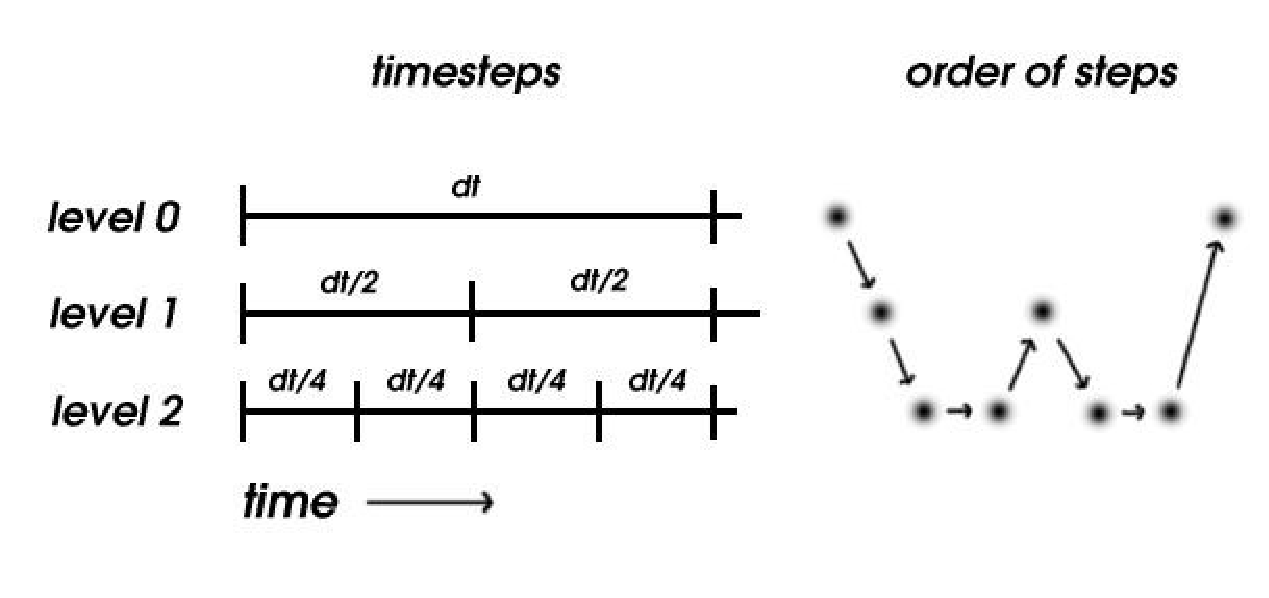
\includegraphics[width=0.6\textwidth]{figures/wcycle.eps}
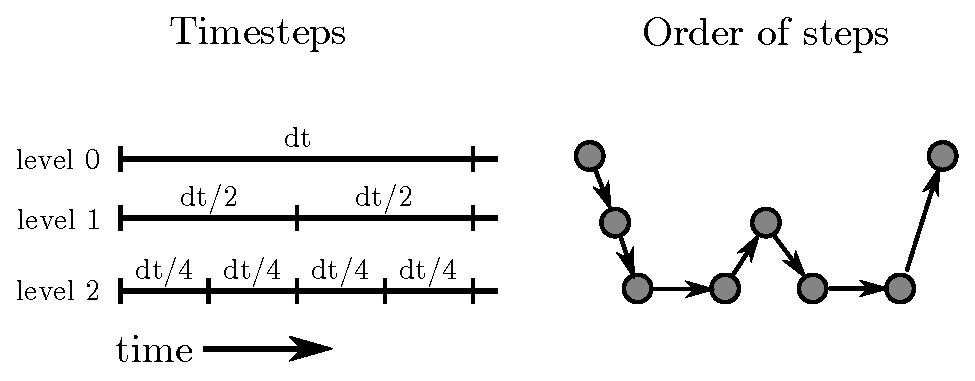
\includegraphics[width=0.6\textwidth]{figures/timestepping.eps}
\end{center}
\caption{\emph{Left:} Example of the timesteps on a 2-level AMR
  hierarchy.  \enzo\ does not restrict the timesteps on the finer levels
  to be a factor of $1/2^n$ smaller.  \emph{Right:} The order in which
  the AMR grids are evaluated on each level.\vspace{1ex}}
\label{fig:wcycle}
\end{figure}

Since interesting regions on the grid may move, the hierarchy must
adapt itself. This happens whenever a level has caught up to its
parent level, by entirely rebuilding the grids on that level and at
finer resolutions. Rebuilding is achieved by applying the grid
refinement criteria to the grids on that level and flagging zones that
require extra grids.  These criteria depend on the physical problem
being simulated; see Section~\ref{sec:refinement_criteria} for more
details.  Once a grid has a set of flagged cells, we apply a
machine-vision based algorithm \citep{Berger91} to find edges and
determine a good placement of subgrids.
%  These subgrids must not overlap one another, must cover all flagged
% cells and their neighbouring cells, and be above a preset efficiency
% threshold, where the efficiency of a cell is defined as the ratio of
% flagged cells to total cells. 
Once these new subgrids have been identified, the solution from the
next coarser grid is interpolated in order to initialize the values on
the new grids.  Finally, any overlap between new subgrids and old ones
is identified, and the prior solution within the regions of overlap is
copied to the new subgrids. This procedure is then repeated on the new
grids and in this way, the entire hierarchy (from the original level
examined and continuing on to all finer levels) is rebuilt.

\subsubsection{(Magneto)-hydrodynamic solver methods}

Four different (magneto)-hydrodynamic methods are implemented in
\enzo: (i) the hydrodynamic-only piecewise parabolic method (PPM)
developed by~\citet{1984JCoPh..54..174C} and extended to cosmology
by~\citet{1995CoPhC..89..149B}; (ii) the MUSCL-like Godunov scheme
\citep{1977JCoPh..23..276V} with or without magnetic fields and Dedner-based
divergence cleaning, described in more detail in
\citet{WangAbelZhang08} and \citet{WangAbel09}; (iii) a constrained
transport staggered MHD scheme \citep{Collins10}, and (iv) the
second-order finite difference hydrodynamics method described in
\zeus~\citep{Stone92a,Stone92b}.

\paragraph{Godunov PPM method (HD only)}

We begin with the direct-Eulerian PPM implementation.  This is an
explicit, higher-order accurate version of Godunov's method for ideal
gas dynamics with the spatially third-order accurate piecewise parabolic monotonic
interpolation and a nonlinear Riemann solver for shock capturing.  It
advances the hydrodynamic equations in the following steps:
%\begin{enumerate}
% \item 
(i) Construct monotonic parabolic interpolation of cell average data,
for each fluid quantity;
% \item 
(ii) Compute interface states by averaging the parabola over the
domain of dependence for each interface;
% \item 
(iii) Use interface data to solve the Riemann problem;
 %\item 
(iv) Difference the interface fluxes to update the cell average
quantities.
%\end{enumerate}

The PPM implementation does an excellent job of capturing strong
shocks across a few cells.  Multidimensional schemes are built up by
directional splitting and produce a method that is formally
second-order accurate in space and time and which explicitly conserves mass,
linear momentum, and energy \citep{Hawley84, Norman86}.  A variety of
Riemann solvers have been implemented.

As described in \citet{1995CoPhC..89..149B}, we modify the method for use in
hypersonic flows when the thermal energy $e$ is extremely small
compared to the total energy $E$.  This situation presents a problem
because in the total energy method the temperature is computed by
subtracting one large number from another (i.e. the kinetic energy
from the total energy), which tends to generate large numerical
inaccuracies. We overcome this difficulty by additionally solving a
thermal energy equation and using $e$ from this equation when we
expect the error to be large.

\paragraph{Godunov MUSCL (HD) with Dedner divergence cleaning (MHD)}
This solver was developed to attack problems in magnetic field
amplification during the formation of galaxies \citep{Wang:2009a} and
to understand the role of proto-stellar jets for the theory of star
formation \citep{Wang:2009b}. It combines the standard approach of
Godunov \citep{Godunov1959} for finite volume techniques with the
method of lines as described by \cite{leveque2002finite} and
\cite{toro-1997}. In addition, it implements the hyperbolic divergence
cleaning algorithm of \cite{2002JCoPh.175..645D}. It supports multiple
approximate Riemann solvers and non-ideal equations of
states. Consequently, this suite of solvers can be used for hydro and
magneto-hydrodynamic simulations. This class of solvers, as
well as a version of the PPM hydro solver, has been ported to
nVidia's CUDA framework, allowing \enzo\ to take advantage of modern
graphics hardware \citep{Wang:2010}.

\paragraph{Godunov MHD with Constrained Transport (MHD)}
This MHD method is second-order in time and space, and preserves the
divergence constraint, $\div \vecB = 0$, to machine precision
through the Constrained Transport (CT) method \citep{Collins10}.  CT, originally
described by \citet{Evans88}, updates the magnetic field with the curl
of an electric field, suitably formulated to preserve $\div
\vecB$.  We employ the CT methods described by \citet{Balsara99} and
\citet{Gardiner05} with the second-order hyperbolic
solver of \citet{Li08a} and the divergence free AMR scheme of
\citet{Balsara01}.

\paragraph{Second-order finite difference method (HD only)}

Lastly, we briefly describe the \zeus\ method, a finite difference
algorithm originally used in the \zeus\ code \citep{Stone92a}. Note
that \enzo\ is entirely independent of the \zeus\ code, and only the
hydrodynamical algorithm of \zeus\ has been implemented in \enzo; the
MHD and radiation-hydrodynamics schemes have not. The \zeus\ method
uses a staggered mesh such that velocities are face-centered, while
density and internal energy are cell-centered.  It splits the solution
up into two steps. The first is the so-called source step, in which
the momentum and energy values are updated to reflect the pressure and
gravity forces, including an artificial viscosity required for
stability. The second step, known as the transport step, accounts for
the advection of conserved quantities (mass, momentum, and energy)
across the grid.

\subsubsection{Gravity}

The current implementation of self-gravity in \enzo\ uses a Fast
Fourier Technique \citep{Hockney88} to solve Poisson's equation on the
root grid on each timestep.  The advantage of using this method is
that it is fast, accurate, and naturally allows both periodic and
isolated boundary conditions for the gravity, choices which are very
common in astrophysics and cosmology.  On subgrids, we interpolate the
boundary conditions from the parent grid (either the root grid or some
other subgrid). The Poisson equation is then solved on every timestep
using a multigrid technique on one subgrid at a time. Aside from
self-consistently calculating the gravitational potential arising from
the baryon fields and particles in the simulation, there are also a
number of options for specifying static gravitational fields, and in
fact including self-gravity is optional.

\subsubsection{N-body Dynamics}

Collisionless matter (e.g. dark matter, stars, etc.) is modeled with
particles that interact with the baryons only via gravity.  These
particles are advanced through a single timestep using a drift-kick-drift
algorithm \citep{Hockney88} to provide second-order accuracy even in
the presence of varying timesteps.  Since the particles follow the
collapse of structure, they are not adaptively refined.  Nor are there
duplicate sets of particles for each level; instead, each particle is
associated with the highest refined level available at its position in
the domain and particles are moved between grids as the hierarchy is
rebuilt. Thus a particle has the same timestep and feels the same
gravitational force as a grid at that refinement level.

Although the particles are fixed in mass once initialized (with the
exception of star particles, which can lose mass in the feedback
process), we can create them with any initial set of masses and
positions.  For example, in many cosmological simulations static
subgrids are included from the beginning in order to improve the
initial spatial and baryonic mass resolution, and these subgrid are
populated with lower mass particles to correspondingly improve the
collisionless mass resolution.
%% One particle per initial grid point seems to provide approximately
%% equal sampling between the dark matter and gas. \mqk{This
%% contradicts the conclusions of O'Shea et al. 2005 that an initial
%% grid twice as fine as the mean particle separation is necessary to
%% properly capture the abundance of low mass halos.}

\subsubsection{Chemistry}
\label{sec.ov.chem}

\enzo\ includes the capability of following up to 12 particle species
using a non-equilibrium chemical network.  The species can be turned
on in sets, with the simplest model including just atomic hydrogen and
helium (H, H$^+$, He, He$^+$, He$^{++}$, e$^-$), and more complete
models adding first species important for gas-phase molecular hydrogen
formation (H$^-$, H$_2$ and H$_2^+$), and then HD formation (HD, D,
D$^+$).
%(We note that a reduced version
%of the chemistry, used only with the flux-limited diffusion radiation
%transport, includes only hydrogen species.)
The cooling and heating due to these species is included (see the next
section). The solution of the rate equations is carried out using one
Jacobi iteration of an implicit Euler time discretization to ensure
stability. To ensure accuracy the rate equations are sub-cycled
within one hydrodynamic timestep, subject to the constraint that the
electron and neutral fractions do not change by more than 10\% in one
sub-cycle.

\subsubsection{Radiative Cooling and Heating}

\enzo\ can operate in a number of different modes with regard to
radiative cooling and heating. In the simplest mode, where the
multi-species flag is turned off and no individual chemical species
are tracked, the cooling rate is computed from a
simple temperature-dependent cooling function, taken from
\citet{SW87}.  If chemistry is turned on, then the code can include
cooling from all species of hydrogen and helium (including H$_2$) --
and the primordial cooling rates are computed in the same Jacobi iteration as the
chemistry.  It is also possible to include metal cooling based on a
set of multi-dimensional lookup tables computed with the
\textsc{Cloudy} code \citep{1998PASP..110..761F} as described in
\citet{2008MNRAS.385.1443S} and \citet{2011ApJ...731....6S}. Note that
the cooling and heating is most commonly treated in the optically-thin
limit, but the code can also follow radiative transfer in a limited
set of energy bins.

\subsubsection{Homogeneous radiation backgrounds}

The chemical networks and heating rates described in the previous
sections can be affected by external radiation fields, and the code
includes a number of pre-calculated meta-galactic UV radiation
backgrounds that are uniform in space but can vary in time.  These are
generally based on the redshift-dependent rates given in
\citet{1996ApJ...461...20H} and \citet{2012ApJ...746..125H}, but can
also include a uniform H$_2$ photo-dissociating background that is
either constant in time or varying as in \citet{WiseAbel05}.

\subsubsection{Radiation transport: ray tracing}

\enzo\ includes a photon-conserving radiative transfer algorithm that
is based on an adaptive ray-tracing method utilizing the HEALPix
pixelization of a sphere \citep{Abel02_RT}. Photons are integrated
outwards from sources using an adaptive timestepping scheme that
preserves accuracy in ionization fronts even in the optically-thin
limit. This has been coupled to the chemistry and cooling network to
provide ionization and heating rates on a cell-by-cell basis. The
method is described in detail (including numerous code tests) in
\citet{Wise11_Moray}.

\subsubsection{Radiation transport: Flux-limited diffusion}

A second option for radiative transfer is a moment-based method that
adds an additional field tracking the radiation energy density.  This
field is evolved using the flux-limited diffusion method, which
transitions smoothly between streaming (optically thin) and opaque
limits and is coupled to an ionization network of either purely
hydrogen, or both hydrogen and helium.  The
resulting set of linear equations is solved using the parallel HYPRE
framework.  Full details on the \enzo\ implementation of this method
can be found in \citet{ReynoldsHayesPaschosNorman2009}.

\subsubsection{Heat Conduction}

Heat conduction, both isotropic and anisotropic, can be included using
a sub-cycled, operator-split method.  The heat fluxes are computed
with simple second-order accurate finite differences, and stability is
ensured by restricting the timestep and using flux-limiters where
appropriate.

\subsubsection{Star Formation and Feedback}

A family of simple heuristic methods are used to model the formation
of stars and their feedback of metals and energy into the gas.  These
methods are based on the work of \citet{CO1992}, and involve the
identification of plausible sites of star formation based on a set of
criteria (for example, dense gas with a short cooling time, which is
both collapsing and unstable).  The local star formation rate is
computed using a range of methods, such as a density-dependent method
based on the Schmidt-Kennicutt relation \citep{K89}.  The affected gas
is converted into a star particle over a few dynamical times, and
metals and thermal energy are injected into the region surrounding the
star particle.  A related set of methods involves the simulation of
single Population III stars, rather than ensembles, and is calibrated
by \textit{ab initio} simulations of primordial star formation.

\subsubsection{Timestep constraints}

All grids on a given level are advanced with the same timestep.  This
time step is determined by first calculating the largest time step
allowed for each cell and for each physical process separately (except
for chemistry and heat conduction, which are sub-cycled).  The level
is then advanced with a timestep equal to the minimum over all of
these $\Delta t$.

%%% Local Variables:
%%% mode: latex
%%% TeX-master: "ms"
%%% End: 


%% Section: numerical methods
\section{Numerical Methods}
\label{sec.methods}

We now describe each of the numerical methods in detail.  The structure of this section mirrors the previous one, in which each method was briefly described; here we present the details.

\input{numerical-amr}
In this section, we describe the four solvers that we have implemented
for solving the fluid equations.  We describe the PPM method in
considerably more detail than the other methods in part because its
implementation in Enzo has not previously been described, but mostly
because it introduces many of the ideas and methods used for the
MUSCL-Dedner and MHDCT schemes (including expansion terms,
reconstruction, Riemann solvers, and dual energy formalism).

\subsection{Hydrodynamics: The PPM method}
\label{sec.hydro.ppm}

One (purely) hydrodynamic method used in \enzo\ is closely based on
the piecewise parabolic method (PPM) of \citet{1984JCoPh..54..174C} --
henceforth referred to as CW84 -- which has been modified for the
study of cosmological fluid flows.  CW84 describe two variants on this
method: Lagrangian Remap and Direct Eulerian.  We use the Direct
Eulerian version in \enzo, which is better suited for AMR simulations.
The Lagrangian Remap version has previously been adapted for
cosmological use as described in \citet{1995CoPhC..89..149B}, and the
implementation we use here is closely based on that work.

The first term on the right hand side of equations~(\ref{eq:momentum})
and (\ref{eq:total_energy}) comes from our choice of comoving
coordinates (a similar term also appears in
equation~(\ref{eq:dm_velocity}), the velocity relation for the dark
matter particles).  A similar term does not appear in the mass
conservation equation (\ref{eq:mass}) because of the comoving density
definition.  We note that these expansion terms could be eliminated
entirely by the proper choice of variables (including time), although
we have not done so here as they do not constitute a major source of
error.  We solve these terms using the same technique -- they are
split from the rest of the terms and solved using an (implicit)
time-centered method, which is straightforward as there are no spatial
gradients.  Note that we use this method for all four of the hydro
solvers.

The remainder of the terms in the fluid equations involve derivatives.
Because we are interested in phenomena with no special geometry, we
will restrict discussion to Cartesian coordinates.  We can
dimensionally split the equations and rewrite the one-dimensional
(Eulerian) versions of
equations~(\ref{eq:mass})--(\ref{eq:total_energy}) without expansion
terms in conservative form as,
\begin{eqnarray}
\frac{\partial \rho}{\partial t}  + \frac{1}{a} \frac{\partial \rho v }{\partial x}    & = &  
     0 \label{eq:mass1d} \\
\frac{\partial \rho v}{\partial t}  + \frac{1}{a} \frac{\partial \rho v^2}{\partial x}   + 
      \frac{1}{a} \frac{\partial p}{ \partial x} & = & 
      \rho \frac{g}{a}  \label{eq:momentum1d}  \\
\frac{\partial \rho E}{\partial t}  + \frac{1}{a} \frac{\partial \rho v E}{\partial x}  & =  &
      \rho v \frac{g}{a} \label{eq:total_energy1d}
\end{eqnarray}
%
Here $x$ and $v$ refer to the one dimensional comoving position and 
peculiar velocity of the baryonic gas, and $g$ is the acceleration at the cell center.
These equations are now in a form that can be solved by the split PPM scheme.

% ------------------------------------------------------------

We now restrict ourselves to the solution of equations
(\ref{eq:mass1d})--(\ref{eq:total_energy1d}) in one dimension.  In the
Direct Eulerian version of PPM, this is accomplished by a three-step
process.  First, we compute effective left and right states at each
grid boundary by constructing a piecewise parabolic description of the
primative variables ($\rho$, $u$ and $E$) and then averaging over the
regions corresponding to the distance each characteristic wave can
travel ($u$, $u-c_s$ and $u+c_s$, where $c_s$ is the sound speed).
Second, a Riemann problem is solved using these effective left and
right states, and finally the fluxes are computed based on the
solution to this Riemann problem and the conserved quantities are
updated.  This is described in detail in CW84, but we will briefly
outline the procedure here both for completeness and to put the
changes we will make in context.

The Eulerian difference equations are:
%
\newcommand{\avp}[1]{\overline{#1}_{j+1/2}}
\newcommand{\avm}[1]{\overline{#1}_{j-1/2}}
\begin{equation}
\rho_j^{n+1} = \rho_j^{n} + \Delta t \left( 
                      \frac{ \avp{\rho}\avp{v} -  \avm{\rho}\avm{v} } {\Delta x_j}
            \right)
     \label{eq:mass_diff}
\end{equation}
\begin{equation}
\rho_j^{n+1} v_{j}^{n+1} =
       \rho_j^{n+1} v_j^n  + \Delta t \left(
          \frac{ \avp{\rho} \avp{v}^2 - \avm{\rho} \avm{v}^2 + \avp{p} - \avm{p}} {\Delta x_j}
             \right)
     + \frac{ \Delta t }{2} g_j^{n+1/2} (\rho_j^n + \rho_j^{n+1}), 
     \label{eq:momentum_diff}
\end{equation}
\begin{eqnarray}
\rho_j^{n+1} E_j^{n+1}  = 
       \rho_j^n E_j^n  & + & \Delta t  \left(
            \frac{  \avp{\rho} \avp{v} \avp{E}  - \avm{\rho} \avm{v} \avm{E}  +
                       \avp{v} \avp{p}    - \avm{v} \avm{p} } {\Delta x_j}
             \right) \nonumber \\
         & & + \frac{ \Delta t }{2} g_j^{n+1/2} (\rho_j^n v_j^n + \rho_j^{n+1} v_j^{n+1} ).
     \label{eq:energy_diff}
\end{eqnarray}

We have used subscripts to indicate zone-centered ($j$) and
face-centered ($j+1/2$) quantities, while superscripts refer to
position in time.  The cell width is $\Delta x_j$.  Although they have
been discretized in space, the accuracy of the updates depend on how
well we can compute the fluxes into and out of the cell during $\Delta
t$.  This in turn depends on our ability to compute the time-averaged
values of $p$, $\rho$ and $v$ at the cell interfaces, denoted here by
$\overline{p}_{j\pm 1/2}$, $\overline{\rho}_{j\pm 1/2}$, and
$\overline{v}_{j\pm 1/2}$.  We now describe the steps required to
compute these quantities.

We first construct monotonic piecewise parabolic (third-order)
interpolations in one dimension for each of $p$, $\rho$, and $v$.  The
pressure is determined from equation~(\ref{eq:eq_of_state}), the
equation of state.  The interpolation formula for some quantity $q$ is
given by:
%
\begin{eqnarray}
q_j(x) & = &  q_{L,j} + \tilde{x}(\Delta q_j + q_{6,j}(1-\tilde{x})), \\
\tilde{x}      & \equiv & {x - x_{j-1/2} \over \Delta x_j}, \qquad
             x_{j-1/2} \leq x \leq x_{j+1/2}. \nonumber
\end{eqnarray}
%
This is equation~(1.4) of CW84 (in the spatial rather than mass
coordinate, as is appropriate for the direct Eulerian approach).  The
quantities $q_{L,j}$, $\Delta q_j$, and $q_{6,j}$ can be viewed simply
as interpolation constants; however, they also have more intuitive
meanings.  For example, $q_{L,j}$ is the value of $q$ at the left edge
of zone j, while $\Delta q_j$ and $q_{6,j}$ are analogous to the slope
and first-order correction to the slope of $q$ (see CW84 for a
complete discussion):
\begin{equation}
\Delta q_j \equiv q_{R,j} - q_{L,j} \qquad 
q_{6,j}    \equiv 6\left[q_j - 1/2\left(q_{L,j} + q_{R,j}\right)\right].
\end{equation}

We have reduced the problem to finding $q_{L,j}$ and $q_{R,j}$.  While
this is simple in principle, it is complicated somewhat by the
requirement that these values be of sufficient accuracy and that the
resulting distribution be monotonic.  That is, no new maxima or minima
are introduced.  The resulting formulae are straightforward but
complicated and are not reproduced here, but see Equations 1.7 to 1.10
of CW84.  We also optionally allow steepening as described in that
reference.

Once we have the reconstruction, the primary quantities ($p$, $\rho$,
$v$ and $E$) are averaged over the domains corresponding to the three
characteristics $u-c$, $u$, or $u+c$ (where $c$ is the sound speed in
a cell).  The linearized gas dynamics equations are then used to
compute second-order accurate left and right states that take into
account the multiple wave families.  This process is described in CW84
and we use their equations (3.6) and (3.7).

With these effective states, an approximation to the Riemann problem
is found (see below for more detail about the Riemann solvers used),
producing estimates for $\overline{p}_{j\pm 1/2}$,
$\overline{\rho}_{j\pm1/2}$, and $\overline{v}_{j\pm 1/2}$ that are
third-order accurate in space and second-order accurate in time.
These are then used to solve the difference Equations
(\ref{eq:mass_diff})--(\ref{eq:energy_diff}) for $\rho^{n+1}$,
$v^{n+1}$, and $E^{n+1}$.

We include an optional diffusive flux (and flattening for the
parabolic curves) that can improve the solution in some cases.  Our
implementation follows that in the appendix of CW84.

In addition, as discussed earlier, the three-dimensional scheme is
achieved by operator-splitting and repeating the above procedure in
the other two orthogonal directions.  The transverse velocities and
any additional passive quantities are naturally and easily added to
this system (see Equation 3.6 of CW84).  

We note that the acceleration required in
Equation~(\ref{eq:momentum_diff}) is actually the acceleration felt by
the entire zone and not just at the zone center.  Therefore, it is
possible to find the mass-weighted average acceleration over the zone
by expanding the density and acceleration distributions and retaining
all terms up to second-order in $\Delta x$
\citep{1995CoPhC..89..149B}, although we find that the potential is so
slowly varying that this is unnecessary.

% ------------------------------------------------------------

\subsubsection{The dual energy formulation for  very high Mach flows} % 2.4

The system described thus far works well for gravitating systems with
reasonable Mach numbers ($<100$) as long as the structures are well
resolved.  This section and the next detail changes that are required
to correctly account for situations where one or both of these
requirements are not met.

Large, hypersonic bulk flows appear to be very common in cosmological
simulations and they present a problem because of the high ratio of
kinetic energy $E_k$ to gas internal energy $e$, which can reach as
high as $10^8$.  Inverted, we see that the internal energy consists of
an extremely small portion of the total energy.  In such a situation,
the pressure, proportional to $E - E_{k}$, is the small difference
between two large numbers: a disastrous numerical situation.  This is
not as large a problem as it may at first appear because it only
occurs when the pressure is negligibly small.  Therefore, even if we
suffer large errors in the pressure distribution in these regions, the
dynamics and total energy budget of the flow will remain unaffected.
Nevertheless, if the temperature distribution is required for other
reasons (e.g., for calculating radiative processes), a remedy is
required.

To overcome this, we also solve the internal energy equation:
\begin{equation}
 \frac{\partial e}{\partial t} 
           + \frac{1}{a} \vecv \cdot \grad e
%         = - \frac{3(\gamma -1)\dot{a}}{a} e
         = - 3 \frac{\dot{a}}{a} \frac{p}{\rho}
           - \frac{p}{a\rho} \div \vecv
\end{equation}
in comoving coordinates.  The structure is similar to the total energy
equation; the second term on the left hand side represents transport,
while the first term on the right is due to expansion of the
coordinate system.  It is differenced (again, in Eulerian form without
the expansion term) as,
%
\begin{equation}
\rho_j^{n+1} e_j^{n+1}  = 
       \rho_j^n e_j^n   +  \Delta t  \left(
            \frac{  \avp{\rho} \avp{v} \avp{e}  - \avm{\rho} \avm{v} \avm{e}} {\Delta x_j} \right)
            - \Delta t \ p_j^{n} \left( \frac{ \avp{v} - \avm{v}} {\Delta x_j} 
                      \right)
                  \label{eq:gasenergy_diff}
\end{equation}
%
Note that because of the structure of this equation, it is not in
flux-conservative form.  In particular, the pressure is evaluated at
the cell center.  Unfortunately, time-centering of this pressure has
proved difficult to do without generating large errors in the internal
energy and so we leave the pressure at the old time in this difference
equation.  This leads to some spreading of shocks; however, we note
that this equation is only used in hypersonic flows.

It is necessary, however, to conserve the total energy so that the
conversion of kinetic to thermal energy is performed properly.  We
must therefore combine the two formulations without allowing the
separately-advected internal energy $e$ to play a role in the gas
dynamics.  This is done by carrying both terms through the simulation
and using the total energy $E$ for hydrodynamic routines and the
internal energy $e$ when the temperature profile is required.  One way
to view this procedure is to treat $e$ as enhanced precision (extra
digits) for $E$ that automatically `floats' to where it is needed.  We
only require that they be kept synchronized when the two levels of
precision overlap.

When the pressure is required solely for dynamic purposes, the 
selection criterion 
operates on a cell by cell basis using,
\begin{equation}
p = \cases{ \rho(\gamma - 1)(E - \vecv^2/2),& 
                  $  (E - \vecv^2/2)/E > {\eta}_1 $; \cr
            \rho(\gamma -1)e,&
                  $  (E - \vecv^2/2)/E < {\eta}_1 $. \cr}
\end{equation}

It should be stressed that as long as the parameter ${\eta}_1$ is
small enough the dual energy method {\it will have no dynamical
effect}.  We use ${\eta}_1 = 10^{-3}$, which is consistent with the
truncation error of the scheme for grid sizes that are typically used
in our simulations.  We are now free to select the method by which the
internal energy field variable $e$ is updated so that it will not
become contaminated with errors advected by the total energy
formulation but still give the correct distribution in shocked
regions.  Since we are concerned with the advection of errors, the
selection criterion must look at each cell's local neighbourhood.  In
one dimension, this is done with,

\begin{equation}
e = \cases{ (E - \vecv^2/2),& $\rho(E - \vecv^2/2)/
    \max ({\rho}_{j-1}E_{j-1},{\rho}_j E_j,{\rho}_{j+1}E_{j+1}) > {\eta}_2$,\cr
            e,& $\rho(E - \vecv^2/2)/
    \max ({\rho}_{j-1}E_{j-1},{\rho}_j E_j,{\rho}_{j+1}E_{j+1}) < {\eta}_2$.\cr}
    \label{eq:dualselect}
\end{equation}

Thus, ${\eta}_2$ determines when the synchronization (of $e$ with $E$)
occurs.  Too high a value may mask relatively weak shocks, while
spurious heating (via contamination) may occur if it is set too low.
After some experimentation, we have chosen ${\eta}_2 = 0.1$, a
somewhat conservative value.  This scheme is optional and is generally
only required in large-scale cosmological simulations where the gas
cools due to the expansion of the universe but large bulk flows
develop due to the formation of structure.

We note that others have independently developed a similar but
distinct scheme for dealing with this problem, which is endemic to
methods adopting the total energy equation.  In \citet{TVD93}, the two
variables adopted are total energy and entropy (rather than total
energy and thermal energy), with an analogous scheme for choosing
which variable to employ.

\subsubsection{Riemann Solvers and Fallback}
\label{sec.riemann}

In this section, we describe the methods we adopt to solve the Riemann
problem, which is generally required to compute the fluxes in any
Godunov-based scheme.  This section therefore applies to all three of
our Godunov-based schemes.  The Riemann problem we are solving
involves two constant states separated by a single discontinuity at
$t=0$.  The subsequent evolution has an exact analytic solution.  This
solution is described in detail in many texts on computational fluid
dynamics \citep[e.g.,][]{toro-1997}.  In brief, there are three waves
that propagate away from the initial discontinuity.  The central wave,
characterized by a density jump but not a pressure jump, is called the
contact discontinuity.  The waves traveling to the left and right of
the contact discontinuity can be either shocks, if characteristics
converge on the wave front, or rarefaction fans if characteristics
diverge.

While there exists an exact solution to this problem, finding it is
expensive.  There are four possible combination of left- and right-
traveling shocks and rarefactions, only one of which is fully
consistent with the initial conditions.  Once the correct physical
state is determined, the pressure in the central region can only be
computed by finding the root to an algebraic equation, which is
necessarily an iterative process.  Thus a series of \emph{approximate}
Riemann solvers are typically used.  There are four approximate
Riemann solvers in \enzo: two-shock \citep{toro-1997}, Harten-Lax-van
Leer \citep[HLL,][]{toro-1997}, HLL with a contact discontinuity
\citep[HLLC,][]{toro-1997}, and HLL with multiple discontinuities
\citep[HLLD,][]{Miyoshi05}.  Two-shock is used only with the PPM
method.  HLL and HLLC are used with PPM, MUSCL (both with and without
MHD) and MHD-CT.  HLLD is exclusively an MHD solver, and works with
both the MUSCL and MHD-CT methods.

The only approximation that two-shock makes is that both left- and
right-moving waves are shocks.  This solution still requires an
iterative method for finding the pressure in between the two waves.
The HLL method alleviates this iteration by assuming that there is no
central contact discontinuity, and the signal speed in the central
region is approximated by an average over the left- and right- moving
waves.  This method is significantly faster than the two-shock method,
but it is also quite a bit more dissipative.  The HLLC is a three-wave
method that improves upon the HLL method by also including the third
wave, the contact discontinuity.

For the MHD equations, there are seven waves instead of three.  This
makes the exact solution to the Riemann problem quite a bit more
expensive.  Both the HLL and HLLC approximations can be formulated for
the MHD equations, and are employed in both the Dedner and CT solvers
in \enzo.  The HLLD solver includes two of the additional waves, the
rotational discontinuities, making it a five-wave solver.

On rare occasions, high-order solutions can cause negative densities
or energies.  Both our PPM and MUSCL solvers employ a Riemann solver
fallback mechanism \citep{Lemaster09}.  If a negative density is found
at a particular interface, the more diffusive HLL Riemann solver is
used to compute the fluxes associated with that cell, and the flux
update is repeated.




\input{numerical-zeus}
\subsection{Gravity: Solving the Poisson Equations}
\label{sec.gravity}



There are multiple methods to compute the gravitational potential (which is an elliptic equation in the Newtonian limit) in a structured AMR framework.  One way would be to model the dark matter (or other collisionless particle-like objects, such as stars) as a second fluid in addition to the baryonic fluid and solve the collisionless Boltzmann equation, which follows the evolution of the fluid density in six-dimensional phase space.  However, this is computationally prohibitive owing to the large dimensionality of the problem, making this approach unappealing for the cosmological AMR code.

The dark matter particles are distributed onto the grids using the cloud-in-cell (CIC) interpolation technique to form a spatially discretized density field (analogous to the baryon densities used to calculate the equations of hydrodynamics).  After sampling dark matter density onto the grid and adding baryon density if it exists (to get the total matter density in each cell), the gravitational potential is calculated on the periodic root grid using a fast Fourier transform.  For periodic boundary conditions, we can use either a simple Greens function kernel of $-k^{-2}$, or the finite-difference equivalent \citep{HockneyEastwoord1980}:
\begin{equation}
G(\vec{k}) = - \frac{\Delta x}{2 \left( sin(k_x \Delta x/2)^2 + sin(k_y \Delta y/2)^2 + sin(k_z \Delta z/2)^2 \right) }
\end{equation}
where $k^2 = k_x^2 + k_y^2 + k_z^2$ is the wavenumber in Fourier space and the potential is calculated in k-space as usual with $\tilde{\phi}(k) = G(k) \tilde{\rho}(k)$.  

For isolated boundary conditions, we use James method (REF).  In this case, the Greens function is generated in real-space so as to have the correct zero-padding properties and then transformed into the Fourier domain.

In order to calculate more accurate potentials on subgrids, \enzo\ re-samples the dark matter density onto individual subgrids using the same CIC method as on the root grid, but at higher spatial resolution (and again adding baryon densities if applicable). Boundary conditions are then interpolated from the potential values on the parent grid.  We use either tri-linear interpolation or a natural second-order spline: both methods seem to give similar results. The potential equation on each subgrid is then solved with the given Dirichlet boundary conditions.  This solution is done with a multigrid relaxation technique (but only applied to each subgrid).

The region immediately next to the boundary can contain unwanted oscillations (Anninos \etal REF), and so we use an expanded buffer zone around the grid, of size three root grid boundary zones (so typically six refined zones).  The density is computed in this region and the potential solved, but only the region which overlaps with the grid itself is used to calculate accelerations.

It is known (REF) that simply interpolating the potential without feeding it back to higher levels leads to errors in the potential at more refined levels because of the build-up of errors during the interpolation of coarse boundary values.  
In addition, neighboring subgrids are not guaranteed to generate the same potential values because of the lack of a coherent potential solve across the whole hierarchy. In an attempt to partially alleviate this problem, we allow for an iterative procedure across sibling grids, in which the potential values on the boundary of grids can be updated with the potential in `active' regions of neighboring subgrids.  To prevent overshoot, we average the potential on the boundary and allow for (typically) 4 iterations.  This procedure can help in many cases, but does not produce a coherent solution across all grids and so does not solve the problem; we are working on a slower but more accurate method which does a multi-grid solve across the whole grid (Reynolds \etal, in preparation).

Forces are computed on the mesh by finite-differencing potential values and are then interpolated to the particle positions, where they are used to update the particle's position and velocity information.  Potentials on child grids are computed recursively and particle positions are updated using the same timestep as in the hydrodynamic equations.  

At this point it is useful to emphasize that the effective force resolution of an adaptive particle-mesh calculation is approximately twice as coarse as the grid spacing at a given level of resolution.  
%The potential is solved in each grid cell; however, the quantity of interest, namely the acceleration, is the gradient of the potential, and hence two potential values are required to calculate this.  In addition, it should be noted that the adaptive particle-mesh technique described here is very memory intensive: in order to ensure reasonably accurate force resolution at grid edges the multigrid relaxation method used in the code requires a layer of ghost zones which is very deep -- typically 6 cells in every direction around the edge of a grid patch.  This greatly adds to the memory requirements of the simulation, particularly because subgrids are typically small (on the order of $12^3 - 16^3$ real cells for a standard cosmological calculation) and ghost zones can dominate the memory and computational 
requirements of the code.


\subsection{N-body Dynamics}
\label{sec.ov.nbody}

The codes needs to be able to model collisionless 
One way would be to model the dark matter (or other collisionless particle-like objects, such as stars) as a second fluid in addition to the baryonic fluid and solve the collisionless Boltzmann equation, which follows the evolution of the fluid density in six-dimensional phase space.  However, this is computationally prohibitive owing to the large dimensionality of the problem, making this approach  unappealing for the cosmological AMR code.
%GB: removed the above (good discussion but not really appropriate in this paper I think, or maybe at the beginning)

To solve the, \enzo\ uses a particle-mesh N-body method to calculate 
the dynamics of collisionless systems \citep{Hockney88}.  This method 
follows trajectories 
of a representative sample of individual particles and is much more 
efficient than a direct solution of the Boltzmann equation in most 
astrophysical situations. 
The gravitational potential is computed by solving the elliptic 
Poisson's equation (Eq.~\ref{eq:potential}).

\begin{eqnarray}
\label{eqn.driftkick}
x^{n+1/2} & = & x^n + (\Delta t/2) v^{n} \nonumber \\
v^{n+1} & = & v^n + \Delta t a^{n+1/2} \\
x^{n+1} & = & x^{n+1/2} + (\Delta t/2) v^{n+1} \nonumber
\end{eqnarray}



Particles are stored in the most highly refined grid patch at the point in space where they exist, and particles which move out of a subgrid patch are sent to the grid patch covering the adjacent volume with the finest spatial resolution, which may be of the same spatial resolution, coarser, or finer than the grid patch that the particles are moved from.  This takes place in a communication process at the end of each timestep on a level.


\subsection{Chemistry}
\label{sec.num.chemistry}

While it is often safe to assume that species (both chemical and
ionization) within a gas can be treated as being in 
equilibrium, in some regimes that are found in astrophysics this is not true.  For example, the cooling and collapse of primordial gas in Population III
star formation is dominated by molecular hydrogen, which in the
absence of dust forms via an inefficient pair of collisional processes
that depend heavily on the local population of free electrons.  
As a
result, when modeling primordial star formation, it is critical to
follow the non-equilibrium evolution of the chemical species of
hydrogen, including molecular hydrogen and deuterium.

The primordial non-equilibrium chemistry routines used in \enzo\ were
first described by Abel et al. and Anninos et
al. \citep{abel97,anninos97}, but have been extended since then with
updated reaction rates and the inclusion of deuterium species.  These 
routines follow the non-equilibrium chemistry of a 
gas of primordial composition with 12 total species:  
$H$, $H^+$, $He$, $He^+$, $He^{++}$, $H^-$, $H_2^+$, $H_2$, $e^-$,
$D$, $D^+$, and $HD$.  (A separate, but related, module follows the
radiative heating and cooling of the gas from atomic and molecular line excitation,
recombination, collisional excitation, free-free transitions, Compton
scattering of the cosmic microwave background, as well as several
models for a metagalactic UV background that heat the gas via
photoionization and discussion -- see Section~\ref{sec.num.cooling}
for more details).  Depending on user parameters, one can follow
simply atomic species ($H$, $H^+$, $He$, $He^+$, $He^{++}$,  and
$e^-$), include those relevant for molecular hydrogen formation
($H_2$, $H_2^+$, and $H^-$), and further include deuterium and its
species ($D$, $D^+$, and $HD$).  
\red{A total of 9 kinetic equations are solved, including 29 kinetic and radiative 
processes, for the 9 species mentioned above.  See Table~\ref{table.collisional} 
for the collisional processes and Table~\ref{table.radiative} for the 
radiative processes solved.}

The chemical reaction equation network is technically challenging to solve due to 
the huge range of reaction timescales involved -- the characteristic creation
and destruction timescales of the various species and reactions can differ by 
many orders of magnitude.  As a result, the set of rate equations is extremely 
stiff, and an explicit scheme for integration of the rate equations can be 
exceptionally costly if small enough timesteps are taken to keep the network
stable.  This makes an implicit scheme much more preferable for such a set of 
equations.  However, an implicit scheme typically require an iterative 
procedure to converge, and for large networks (such as this one) an implicit
method can be very time-consuming, making it undesirable for a large, three-dimensional
simulation.

\enzo\ solves the rate equations using a method based on a backwards differencing 
formula (BDF) in order to provide a stable and accurate solution.  This technique is
optimized by taking the chemical intermediaries $H^-$ and $H_2^+$, which have 
large rate coefficients and low concentrations, and grouping them into a separate
category of equations.  Due to their fast reactions these species are very sensitive
to small changes in the more abundant species.  However, due to their low overall
concentrations, they do not significantly influence the abundance of species with
higher concentrations.  Therefore, reactions involving these two species can be
decoupled from the rest of the network and treated independently.  In fact, $H^-$ 
and $H_2^+$ are treated as being in equilibrium at all times, independent of 
the other species and the hydrodynamic variables.  This allows a large speedup
in solution as the BDF scheme is then applied only to the slower 7- or
10-species network (depending on whether deuterium is included or not)
on timescales closer to those required by the hydrodynamics of the simulation.
Even so, the accuracy and stability of the scheme is maintained by subcycling the 
rate solver over a single hydrodynamic timestep.  These subcycle timesteps are 
determined so that the maximum fractional change in the electron concentration is
limited to no more than $10\%$ per timestep.

It is important to note the regime in which this model is valid.  According to Abel et al. and
Anninos et al. \citep{abel97,anninos97}, the reaction network is valid for temperatures
between $10^0 - 10^8$ K.  The original model discussed in these two references is only
valid up to $n_H \sim 10^4$~cm$^{-3}$.  However, addition of the 3-body $H_2$ formation
process (equation 20 in Table~\ref{table.collisional}) allows 
correct modeling of the chemistry of the gas up
until the point where collisionally-induced emission from molecular hydrogen becomes an important
cooling process, which occurs at $n_H \sim 10^{14}$~cm$^{-3}$.  A further concern is that
the optically thin approximation for radiative cooling breaks down, which
occurs before $n_H \sim 10^{16} - 10^{17}$~cm$^{-3}$.  Beyond this point, 
modifications the cooling function that take into account the non-negligible
opacity in the gas must be made, as discussed by \citet{2004MNRAS.348.1019R}. 
Even with these modifications, a completely correct description of the cooling of
this gas will require some form of radiation transport, which will greatly 
increase the cost of the simulations.

\red{Several processes are neglected.  The deuterium atom and its processes are 
completely ignored, which may have some effect.  Recent work shows that HD is
a more effective coolant than previously thought~\citep{2005MNRAS.361..850L}.  However,
the fractional abundance of HD is so low that under circumstances relevant to
the formation of a Population III star in an un-ionized region it should be
sub-dominant.  However, the enhanced electron fraction in fossil 
HII regions (as discussed later in this thesis) could result in the HD molecule
becoming a dominant cooling mechanism at relatively low ($\sim$ few hundred K)
temperatures, and could potentially cool the gas down to below $100$~K, which can
enhance fragmentation and could have important consequences for the IMF of 
primordial stars forming in a relic HII region~\citep{2005MNRAS.364.1378N}.}

Aside from deuterium, the chemical reactions involving lithium 
are also neglected.  According to \citet{1998A&A...335..403G}, these are 
not important for the density and temperature regimes explored 
by the simulations discussed in this thesis.  However, at higher densities it 
is possible that there are regimes where lithium can be an important coolant.



%---------------- table of collisional processes

\begin{table}
\begin{center}
{\bfseries Collisional Processes}\\[1ex]
\begin{tabular}{llllllll}
(1) & H & + & e$^-$ & $\rightarrow$ & H$^+$ &+& 2e$^-$ \\
(2) & H$^+$ &+ &e$^-$ & $\rightarrow$ & H &+ &$\gamma$ \\
(3) & He &+& e$^-$ & $\rightarrow$ & He$^+$ &+& 2e$^-$  \\
(4) & He$^+$ &+& e$^-$ & $\rightarrow$ & He &+ &$\gamma$  \\
(5) & He$^{+}$ &+& e$^-$ & $\rightarrow$ & He$^{++}$ &+& 2$e^-$  \\
(6) & He$^{++}$ &+& e$^-$ & $\rightarrow$ & He$^+$ &+& $\gamma$ \\
(7) & H &+& e$^-$ &$\rightarrow$& H$^-$ &+& $\gamma$  \\
(8) & H$^-$ &+& H &$\rightarrow$ & H$_2$ & +& e$^-$ \\
(9) & H &+ &H$^+$ &$\rightarrow$ &H$_2^+$ &+ &$\gamma$ \\
(10) & H$_2^+$ &+ &H &$\rightarrow$ &$H_2$ &+ &$H^+$ \\
(11) & H$_2$ &+ &H$^+$ &$\rightarrow$ &H$_2^+$ & +& H \\
(12) & H$_2$ &+ &e$^-$ & $\rightarrow$ & 2H & + & e$^-$  \\
(13) & H$_2$ & + & H & $\rightarrow$ & 3H &   &      \\
(14) & H$^-$ & + & e$^-$ & $\rightarrow$ & H & + & 2e$^-$ \\
(15) & H$^-$ & + & H & $\rightarrow$ & 2H & + & e$^-$ \\ 
(16) & H$^-$ & + & H$^+$ & $\rightarrow$ & 2H & & \\
(17) & H$^-$ & + & H$^+$ & $\rightarrow$ & H$_2^+$ & + & e$^-$ \\
(18) & H$_2^+$ & + & e$^-$ & $\rightarrow$ & 2H & & \\
(19) & H$_2^+$ & + & H$^-$ & $\rightarrow$ & H$_2$ & + & H  \\
(20) & 3H & & & $\rightarrow$ & H$_2$ & + & H
\end{tabular}
\caption[]{Collisional processes solved in the Enzo nonequilibrium
primordial chemistry routines.}
\label{table.collisional}
\end{center}
\end{table}



\begin{table}
\begin{center}
{\bfseries Radiative Processes}\\[1ex]
\begin{tabular}{llllllll}
(21) & H & + & $\gamma$ & $\rightarrow$ & H$^+$ & + & e$^-$ \\
(22) & He & + & $\gamma$ & $\rightarrow$ & He$^+$ & + & e$^-$ \\
(23) & He$^+$ & + & $\gamma$ & $\rightarrow$ & He$^{++}$ & + & e$^-$ \\
(24) & H$^-$ & + & $\gamma$ & $\rightarrow$ & H & + & e$^-$ \\
(25) & H$_2$ & + & $\gamma$ & $\rightarrow$ & H$_2^+$ & + & e$^-$ \\
(26) & H$_2^+$ & + & $\gamma$ & $\rightarrow$ & H & + & H$^+$ \\
(27) & H$_2^+$ & + & $\gamma$ & $\rightarrow$ & 2H$^+$ & + & e$^-$ \\
(28) & H$_2$ & + & $\gamma$ & $\rightarrow$ & H$_2^*$ & $\rightarrow$ & 2H \\
(29) & H$_2$ & + & $\gamma$ & $\rightarrow$ & 2H &  & 
\end{tabular}
\caption[]{Radiative processes solved in the Enzo nonequilibrium
primordial chemistry routines.}
\label{table.radiative}
\end{center}
\end{table}

\subsection{Star formation and feedback}
\label{sec.ov.star}

\subsubsection{Overview}
% Overview of methodology

While the physics discussed in other sections of this paper is crucial
to the study of cosmological structure formation, most observations of
galaxies in the infrared, optical, and ultraviolet wavelengths are of
stellar populations.  Furthermore, stars eject energy and metal-
enriched gas throughout their lives, drastically modifying their own
environments' cooling properties.  Broadly speaking, the formation of
galaxies and galaxy clusters cannot be completely modeled without
including the feedback of energy and metals from stellar populations.
In particular, it is thought that feedback is crucial for suppressing
the large numbers of dwarf-like galaxies that CDM theories predict
\citep{1991ApJ...381...14L,1991ApJ...379...52W}.  An early burst of
star formation could remove a large fraction of cold gas from such
systems \citep{1978MNRAS.183..341W,1991ApJ...367...45C}.  Also, the
unexpectedly low luminosities of small clusters and groups (relative
to the richest clusters) is commonly explained through feedback
\citep{1991ApJ...383..104K}.  Energy ejected during the formation of
the cluster ellipticals lowers the central density and hence the X-ray
luminosity of such clusters \citep{1997ApJ...484L..21C}.  For all of
these reasons, it is critical to include star formation and the
feedback of energy and metals into the interstellar and intergalactic
media in cosmological simulations.

Modeling star formation in the context of galaxy formation forces one
to confront two fundamental problems. The dynamical range required to
study galaxy formation and evolution is substantial, and attempting to
directly resolve the formation of individual stars in the context of a
Milky Way-type galaxy is computationally unfeasible.  Also, a strong
theoretical understanding of the details of star formation is
currently lacking.  Due to these challenges, models of star formation
in cosmological simulations are largely phenomenological, and the
``stars'' that are formed are in most cases meant to represent an
ensemble stellar population (although not all; see
Section~\ref{sec:starform_pop3}).
% BWO: I use 'phenomenological' right above this, but could probably
% go for 'parametric' or 'heuristic' if people object to my usage.

The \enzo\ code includes approximately ten models for star formation
and feedback.  Broadly speaking, these methods all work in similar
ways: At a specified time interval, all grid cells that are at the
highest local level of refinement (i.e., have no child cells) are
examined to see if they meet a set of criteria for star formation.
This may simply be a baryon density threshold, but may include more
complex tests, such as an examination of local cooling and dynamical
time scales, molecular hydrogen fraction, metallicity, and converging
gas flows.  If the star formation criteria are met, some mass of gas
is taken away from the cell in question and a ``star particle'' with the
same mass is placed in the center of that cell, with the same momentum
vector as the removed gas.  This star particle is then allowed to
inject mass, momentum, thermal energy, metals, and possibly magnetic
fields and/or cosmic ray populations into its local environment.  In
general, the particle is treated as an ensemble of stars, with
feedback properties occuring over time according to the assumed
initial mass function of the stellar population.

In the following sections, we describe some of the more widely-used star formation
and feedback methods used in \enzo.  We note that similar methods have
been employed in many other codes used for galaxy formation, with
comparable implementations for both star formation and feedback in
other grid-based codes.  With regards to particle-based codes, star
formation is broadly similar in implementation, though feedback is
typically implemented in a very different way due to the Lagrangian
nature of the method \citep[see, e.g.,][]{sh03a,sh03b,hs03}.

% Specific example: Cen & Ostriker
\subsubsection{Cen \& Ostriker}
\label{sec:starform_cen}

The Cen \& Ostriker method is a heuristic model of star formation
on galactic scales.  This method, first described by
\citet{CO1992}, assumes that star particles 

s similar in some ways to the Kravtsov algorithm
but has more complex criteria for determining where stars should
be formed.  In this method, cells that form stars must have a 
baryon overdensity higher than some threshold 
$\rho_b/\bar{\rho}_b \geq \eta$ 
where $\rho_b$ is the baryon density in that cell, 
$\bar{\rho_b}$ is the mean baryon density in the simulation,
and $\eta$ is the user-defined overdensity threshold.
Additionally, the gas in the cells must be contracting, 
cooling rapidly, and gravitationally unstable, e.g.:

\begin{equation}
\nabla \cdot \vec{v}_b < 0,
\label{cencont}
\end{equation}

\begin{equation}
t_{cool} < t_{dyn} \equiv \sqrt{3 \pi / 32G \rho_{tot}},
\end{equation}

\begin{equation}
m_{b} > m_{J} \equiv G^{-3/2} \rho_{b}^{-1/2}C^{3}
\left[ 1 + \frac{\delta\rho_{d}}{\delta\rho_{b}} \right]^{-3/2}
\end{equation}

where $\vec{v}$ is the velocity of the gas in the cell, $\rho_{b}$ and 
$\rho_{d}$ are the cell's baryon and dark matter density, respectively,
$\rho_{total} = \rho_{b} + \rho_{d}$, $m_{b}$ and $m_{j}$ are the 
baryonic mass in the cell and jeans mass of the cell, and C is the 
isothermal sound speed in the cell.  
If all of these criteria are met, 
the mass of a star particle is calculated as \(m_{*} = m_{b} 
\frac{ \Delta t}{ t_{dyn} } f_{*eff} \), 
where $f_{*eff}$ is the star formation efficiency parameter.

If $m_{*}$ is greater than a minimum star mass $m_{*min}$, a particle 
is created and given several attributes:  Mass, a unique index number, 
the time of formation $t_{form}$, the local dynamical free-fall time 
$t_{dyn}$ and the metallicity fraction of the baryon gas in the cell 
$f_{Zb}$.  There is a user-defined minimum dynamical time
$T_{dyn,min}$ which is observationally motivated and affects the
feedback rates (see below).
The particle is placed in the center of the cell and given 
the same peculiar velocity as the gas in the cell, and is then treated 
in the same manner as the dark matter particles.  An 
amount of baryon gas corresponding to the new particle's mass is 
removed from the cell.  

In addition, we have added a stochastic star formation algorithm that keeps 
track of all of the sub-mass threshold stars that should have been created 
and when the total mass of uncreated stars is greater than the minimum mass, 
a star particle is created.

The feedback of energy and metals into the baryon gas is similar to
the Kravtsov feedback, with some important differences.  The star formation 
algorithm creates each star particle instantaneously.  However, feedback
should take place over a significant timescale, as all of the stars contained
within the ``star particle'' would form over a long period of time.  Therefore,
we assume that for the purposes of feedback that the mass of stars formed
at a time $t$ with finite timestep $\Delta t$ is:

\begin{eqnarray}  
\Delta m_{sf} =  m_{*} \left[ \left(1 + \frac{t-t_{form}}{t_{dyn}}  \right)
%\nonumber \times \\ % uncomment for 2-column
		   \exp{\left( \frac{-(t-t_{form})}{t_{dyn}} \right) }
%                    \nonumber \\ 
	       - \left( 1 + \frac{t+ \Delta t-t_{form}}{t_{dyn}} \right) 
%	       \nonumber \\ 
                    \exp{ \left( \frac{-(t+\Delta t-t_{form})}{t_{dyn}} \right)  }
                   \right]
\end{eqnarray}

which can be represented more clearly in integral form:

\begin{eqnarray}
\int_{t}^{t+Dt} \frac{dM}{dt} dt = \int_{t}^{t+Dt} m_{*} 
\frac{dt}{t_{tyn}} \left( \frac{t-t_{form}}{t_{dyn}} \right) 
%\nonumber \times \\ 
\exp{ \left( - ~ \frac{t-t_{form}}{t_{dyn}} \right) }
\end{eqnarray}

During this timestep, we assume that the star particle feeds back
metal-enriched gas and thermal energy from supernovae and from stellar winds.
Since massive stars have very short lifetimes, we assume that there is an
immediate feedback of some fraction $f_{SN}$ of the rest energy from the
stars created that timestep into the baryon gas, such that 
$E_{add} = f_{SN} \Delta m_{sf} c^2$, where c is the speed of light.
In addition, a fraction $f_{Z*}$ of the metal from the star particle
is fed back into the baryon gas, which takes into account the effects
of metal recycling.  Finally, a fraction of the mass $f_{m*}$ from all
stars (rather than just supernovae) is fed back into the gas along with
momentum in order to simulate the mass ejection from non-exploding stars
via stellar winds.

There are six user-defined parameters in this algorithm:  three deal with the
star formation ($\eta$, $m_{*min}$ and $T_{dyn,min}$), and three 
deal with feedback ($f_{SN}$, $f_{Z*}$ and $f_{m*}$).  Some of these
parameters are completely free, while others can be guided by observation
or theory.  For example, the supernova feedback parameter, $f_{SN}$, can be 
constrained assuming that, for every $200 M_\odot$ of stars created, one
supernova occurs, and this event feeds back approximately $10^{51}$ ergs of
thermal energy, giving:

\begin{equation}
f_{SN} = \frac{10^{51} ergs}{200~M_\odot c^2} \simeq 3 \times 10^{-6}
\end{equation}

The metal yield $f_{Z*}$, defined as the mass in metals produced per unit
mass of stars created, can be constrained by a theoretical model of
 \citet{1995ApJS..101..181W}.  This model suggests that $f_{Z*} = 0.02$
is an appropriate number.  The minimum dynamical time is set to be $T_{dyn,min} = 10^7$
~years to agree with timescales seen in nearby OB associations.

The other parameters, such as the overdensity threshold $\eta$, minimum star
 mass $m_{*min}$, and mass ejection fraction $f_{m*}$ are not well constrained 
either theoretically or observationally.  Indeed, $m_{*min}$ is a purely
numerical parameter designed to keep the code from producing too many star 
particles, and thus has no observational or theoretical counterpart.  These
parameters have to be set by performing parameter studies and comparing to 
observations.  Unfortunately, the range of parameter space is large, and
the results may be degenerate for some combinations of these parameters.



% Specific example: Kravtsov
\subsubsection{Kravtsov}
\label{sec:starform_kravtsov}

% GB: Is this going to be in the code????
% GB: I assume not, so I am commenting it out.  Text to be used in another paper?

%Kravtsov's method of star formation is designed to reproduce
%the global Schmidt law of star 
%formation~\citep{2003ApJ...590L...1K,1959ApJ...129..243S}.
%This algorithm is deliberately minimal, and is explicitly geared
%towards modeling star formation in a phenomenological way on kiloparsec
%scales.  Stars are assume to form with a characteristic gas timescale 
%$\tau_*$ such that $\dot{\rho}_* = \rho_{gas}/\tau_*$ where $\rho_{gas}$ 
%and $\rho_*$ are the baryon gas and stellar densities, respectively.  
%This ``constant efficiency'' model on the scale of star formation 
%regions is well motivated observationally \citep{1996AJ....112.1903Y,2002ApJ...569..157W}.  
%Star formation is only allowed to take place in very dense regions
%with $\rho_{gas} \geq \rho_{SF}$, where $\rho_{SF}$ is a constant
%proper density threshold above which star formation is allowed to
%occur.  No other criteria are imposed.  Kravtsov's typical choices
%for $\tau_*$ and $\rho_{SF}$ are $\tau_* = 4$ Gyr and $\rho_{SF} =
%1.64~$M$_\odot$~pc$^{-3}$~$(n_H \sim 50$~cm$^{-3})$.  The adopted timescale
%is derived from the observationally-determined normalization of the
%Schmidt law, and the density threshold is determined by observations
%of star forming regions on $\sim 100$ pc scales.  Note that the density
%threshold is in proper, not comoving, units.

%Algorithmically, the star formation events in Kravtsov's code
%are assumed to occur once every global time step 
%$\Delta t_0 \leq 10^7$.  In cells where star formation is
%determined to occur (i.e. $\rho_{gas} \geq \rho_{SF}$) a
%collisionless ``star particle'' is assumed to form, with a 
%mass $m_* = \dot{\rho}_* V_{cell} \Delta t_0$, where
%$\dot{\rho}_*$ is described above and $V_{cell}$ is the 
%volume of the mesh cell.  These star particles are
%formed instantaneously, with all $m_*$ of gas being
%taken out of the cell and immediately deposited into the
%star particle.  This particle is then given the velocity
%of the gas in the cell, and thereafter treated as a 
%collisionless particle.  The \enzo\ implementation
%of this algorithm is similar, except that instead of 
%forming stars only at the root grid time step, we allow 
%stars to form at the time step of the highest level of
%resolution at any particular point in space.  As can be seen
%from the equation for $m_*$ above, this can result in very 
%small stellar masses.  To avoid memory and processor time
%issues related to having very large numbers of star particles
%we impose a threshold mass $M_{*,min}$ such that a star
%particle only forms if $m_* \geq M_{*,min}$.  An
%appropriate choice of $M_{*,min}$ does not significantly 
%change the star overall star formation history of a 
%simulation, though it may delay the onset of star formation 
%in a given cell relative to a simulation without a particle mass
%threshold.

%Each ``star particle'' is assumed to represent an ensemble
%of stars and is treated as a single-age stellar population.
%Kravtsov assumes that the IMF is described by a
%Miller \& Scalo functional form with stellar masses between
%$0.1$ and $100~M_\odot$ \citep{1979ApJS...41..513M}.  All stars in this
%IMF with $M_* > 8~M_\odot$ deposit $2 \times 10^{51}$ ergs of
%thermal energy and a mass $f_z M_*$ of metals into the
%cell in which they form without delay, with
%$f_z \equiv min(0.2, 0.01~M_*-0.06)$ (i.e. instantaneous
%deposition of metals).  The definition of $f_z$ is a rough
%approximation of the results of 
%\citet{1995ApJS..101..181W}.

%Kravtsov reports that simulations with this algorithm
%reliably reproduce the star formation rate-gas surface
%density relation of the Schmidt law, and are not particularly
%sensitive to numerical parameters \citep{2003ApJ...590L...1K}.
%He also notes that this is surprisingly insensitive to
%the presence or absence of feedback and details of the cooling
%and heating properties of the gas, which suggests that the
%global star formation rate is determined by gravitationally-
%driven supersonic turbulence (on large scales)
%rather than stellar feedback or thermal instabilities on small 
%scales.

% Specific example: H2-regulated
\subsubsection{H2-regulated}
\label{sec:starform_H2reg}

% Specific example: Pop III
\subsubsection{Population III}
\label{sec:starform_pop3}



%\subsubsection{The Kravtsov star formation and feedback algorithm}






\subsection{Time Stepping}
\label{sec.timestepping}

%\dcc{Made this its own section (not really part of the AMR, it's more
%  general than that.)  Added stuff on harmonic average for 3d. See
%  note below on acceleration timestep criterion being crap. Moved
%  w-cycle to the previous section}

In \enzo, resolution of the equations being solved is adaptive in time 
as well as in space.  The timestep in \enzo\ is satisfied on a level-by-level
 basis by finding the largest timestep such that multiple criteria are
satisfied on each level.  The timestep criteria used by Enzo are 
(showing the one-dimensional case for clarity):

\begin{equation}
\Delta t_{hydro} = min \left( \kappa_{hydro} \frac{a \Delta x}{c_{s} + |v_x|} \right)_L ,
\label{eqn:dthydro}
\end{equation}

\begin{equation}
\Delta t_{dm} = min \left(\kappa_{dm} \frac{a \Delta x}{v_{dm,x}} \right)_L ,
\label{eqn:dtdarkmatter}
\end{equation}

\begin{equation}
\Delta t_{exp} = f_{exp} \left( \frac{a}{\dot{a}} \right) ,
\label{eqn:dtexpand}
\end{equation}

\begin{equation}
\Delta t_{accel} = min \left( \sqrt{\frac{\Delta x}{\vec{g}}} \right)_L 
\label{eqn:dtaccel}
\end{equation}

 In equations~\ref{eqn:dthydro}-\ref{eqn:dtaccel}, the $min ( \ldots )_L$
formalism means that this value is calculated for all cells on a given level
L and the minimum overall value is taken as the timestep.  
Equation~\ref{eqn:dthydro} ensures that all cells satisfy the 
Courant-Freidrichs-Levy (CFL) condition for accuracy and stability of an explicit
finite difference discretization of the Euler equations.  Effectively this condition
forces the timestep to be small enough such that any changes in the fluid propagate
less than a single grid spacing, $\Delta x$.  In this equation, $\kappa_{hydro}$ is 
a numerical constant with a value of $0 < \kappa_{hydro} \leq 1$ (with a typical
value of $\kappa_{hydro} \sim 0.3-0.5$) that ensures that the CFL condition is always
met, and $c_s$ and $v_x$ are the sound speed and peculiar baryon
velocity in a given cell.

Equation~\ref{eqn:dtdarkmatter} is analogous to Equation~\ref{eqn:dthydro} and ensures
accuracy in the N-body solver by requiring that no dark matter particle travels more than
one cell width.  The parameter $\kappa_{dm}$ is analogous to $\kappa_{dthydro}$, with
an identical range of values.  Equation~\ref{eqn:dtexpand} limits the timestep such 
that the expansion parameter a can only change by a fractional amount of $f_{exp} = \Delta a/a$, 
where $f_{exp}$ is a user-defined parameter and has typical values of $f_{exp} = 0.01-0.02$.
This is required for the stability of the PPM algorithm in comoving coordinates, and
typically limits the timestep only at high redshifts when densities are relatively
homogeneous.

Equation~\ref{eqn:dtaccel} is supplementary to equation~\ref{eqn:dthydro} in that it
takes into account the possibility of large accelerations causing numerical 
instabilities by violating the Courant condition.  In this equation, $\vec{g}$ is the
gravitational acceleration in each cell on level L.  \blue{ \emph{It should be
  noted that the timestep is computed before the acceleration field is computed,
  and the acceleration field is deleted at the end of each time step.
  So this condition isn't ever actually enforced.  We should either
  fix this problem, or not discuss it.
 -dcollins.} }

Equation ~\ref{eqn:dthydro} is valid for one dimension.  For 2 or 3
dimensions, it was shown by \cite{Godunov1959}  that using the
harmonic average of the timestep found along each of the coordinate
axes yields a maximum $\kappa_{hydro} = 0.8$.  So letting $\Delta
t_x$, $\Delta t_y$, and $\Delta t_z$ be the analogues of
eqn. \ref{eqn:dthydro} along the $x,y$ and $z$ axes, 
\begin{equation}
\Delta t_{hydro} = min ( \kappa_{hydro} /( \frac{1}{\Delta t_x}
+\frac{1}{\Delta t_y} + \frac{1}{\Delta t_z} ) )_L
\end{equation}

For all other criteria, multiple dimensions are accounted for by
repeating the one dimensional criterion along each axis, and taking
the minimum.

%\input{numerical-units}

%% Section: software implementation
% \input{software}

%% Section: code tests
%%  this should probably be done with one file per test

%%%%%%%%%%%%%%%%%%%%%%%%%%%%%%%%%%%%%%%%%%%%%%%%%%%%%%%%%%%%%%%%%%%%%%%%%%%%%
\section{Code tests}
\label{sec.tests}

%%%%%%%%%%%%%%%%%%%%%%%%%%%%%%%%%%%%%%%%%%%%%%%%%%%%%%%%%%%%%%%%%%%%%%%%%%%%%
\subsection{Verifying and validating the \enzo\ code}
\label{sec.tests.vandv}

\red{(Britton)} Description of test suite and test runner.

\red{(Brian)} Refer to all code comparisons that Enzo has been part of.

%%%%%%%%%%%%%%%%%%%%%%%%%%%%%%%%%%%%%%%%%%%%%%%%%%%%%%%%%%%%%%%%%%%%%%%%%%%%%
\subsection{Representative test problems}
\label{sec.tests.problems}

General structure for each test problem:  Outline how the test problem is constructed (initial and boundary conditions), 
the analytical solution, why we have in the paper (what does it break, or what flaw does it expose (not in enzo of course)),
a plot showing how well enzo solves said test problem, and a brief description of the plot and how awesome enzo is.

%%%%%%%%%%%%%%%%%%%%%%%%%%%%%%%%%%%%%%%
\subsubsection{Sod Shock Tube}
\label{sec.tests.sodshock}
\red{(Greg)}
Problem type 1.  AMR version.  Tests the hydro.
This is also problem 7.2 in the FLASH method paper.

%%%%%%%%%%%%%%%%%%%%%%%%%%%%%%%%%%%%%%%
\subsubsection{Wave pool}
\label{sec.tests.wavepool}
\red{(Greg)}
Problem type 2, with AMR.  Tests reflections of waves at grid boundaries.

%%%%%%%%%%%%%%%%%%%%%%%%%%%%%%%%%%%%%%%
\subsubsection{Shock pool}
\label{sec.tests.shockpool}
\red{(Greg)}
Problem type 3, with AMR.  Tests passage of shock through a refinement boundary.

%%%%%%%%%%%%%%%%%%%%%%%%%%%%%%%%%%%%%%%
\subsubsection{Double mach reflection}
\label{sec.tests.doublemach}
\red{(Brian)}
Problem type 4.  This is one of Alexei's test problems.  Tests
boundary conditions in hydro.

%%%%%%%%%%%%%%%%%%%%%%%%%%%%%%%%%%%%%%%
\subsubsection{Sedov Explosion}
\label{sec.tests.sedov}
\red{(Elizabeth)}
Problem type 7.  One of Alexei's test problems.  
Also problem 7.4 in the FLASH method paper.
This tests the hydro in the strong-shock limit.

%%%%%%%%%%%%%%%%%%%%%%%%%%%%%%%%%%%%%%%
\subsubsection{Point source gravity test}
\label{sec.test.gravitypointsource}
\red{(Greg)}
This is the TestGravity (problem 23) test problem.  It tests gravity around a point source, using fixed AMR.

%%%%%%%%%%%%%%%%%%%%%%%%%%%%%%%%%%%%%%%
\subsubsection{Orbit Test}
\label{sec.test.testorbit}
\red{(Greg)}
This is the TestOrbit problem (problem 29 for GB).  This tests gravity and particle integration (no hydro).

%%%%%%%%%%%%%%%%%%%%%%%%%%%%%%%%%%%%%%%
\subsubsection{Self-Similar infall test}
\label{sec.tests.infall}
\red{(Greg)}
Problem type 24.  This is a test based on Bertschinger's 1985 3D self-similar infall
solution, and tests gravity + hydro.

%%%%%%%%%%%%%%%%%%%%%%%%%%%%%%%%%%%%%%%
\subsubsection{Zel`Dovich Pancake}
\label{sec.tests.pancake}
\red{(Brian)}
Problem type 20, unigrid and AMR both.  Tests gravity + hydro.

%%%%%%%%%%%%%%%%%%%%%%%%%%%%%%%%%%%%%%%
\subsubsection{Cosmology simulations}
\label{sec.tests.}
\red{(Brian)}
Talk about cosmology code comparisons, where Enzo is good/weak.

%%%%%%%%%%%%%%%%%%%%%%%%%%%%%%%%%%%%%%%
\subsubsection{Representative MHD test}
\label{sec.tests.mhd}
\red{(Dave)}
One representative MHD test.  What's the best/hardest one?

%%%%%%%%%%%%%%%%%%%%%%%%%%%%%%%%%%%%%%%
\subsubsection{1-zone free-fall test}
\label{sec.tests.freefall}
\red{(Britton)}
One zone free fall test.  Tests cooling, chemistry.

%%%%%%%%%%%%%%%%%%%%%%%%%%%%%%%%%%%%%%%
\subsubsection{Representative ray-tracing test}
\label{sec.tests.raytracing}
\red{(John)}
One test for MORAY: best/hardest one!

%%%%%%%%%%%%%%%%%%%%%%%%%%%%%%%%%%%%%%%
\subsubsection{Representative FLD test}
\label{sec.tests.fld}
\red{(Dan)}
One test for the implicit FLD: best/hardest one.




%% Section: parallelism and performance
\section{Parallel Strategy and Performance}
\label{sec.parallel}

\subsection{Parallel Strategy}

% GB to work on this
%  - expand to include better description
%  - include load balancing options

When \enzo\ is run on a distrubuted platform, some of the data is
replicated to all processors, while some remains on a single processor.
A description of the entire hierarchy (the position and size of each grid, as well
some other meta data) is stored on each processor.  This enables each
grid to know what grids are near it in the hierarchy, regardless of
where the data is.  The actual Baryon data (density, velocity, energy,
and any chemistry data) and particle data are stored on only one
processor.  Storing the entire hierarchy on all processor does create
some overhead, but in practice this is not an issue until one reaches
the extremely large scale.
  The code handles load balancing 
on a level-by-level basis such that the workload on each level is 
distributed as uniformly as possible across all processors.  Spatial locality of 
grids is not forced during message passing, for maximum flexibility (though not
necessarily maximum efficiency).  
The MPI message passing library\footnote{http://www-unix.mcs.anl.gov/mpi/}
 is used to transfer data between processors.
 
 


%old text
%Every processor 
%keeps a description of the entire grid hierarchy at all times, so that 
%each processor knows where all grids are.  However, baryon and particle 
%data for a given grid only exists on a single processor.  See 
%Figure~\ref{fig.2.amrhierarchy} for a schematic example of this.  



\begin{figure}
\begin{center}
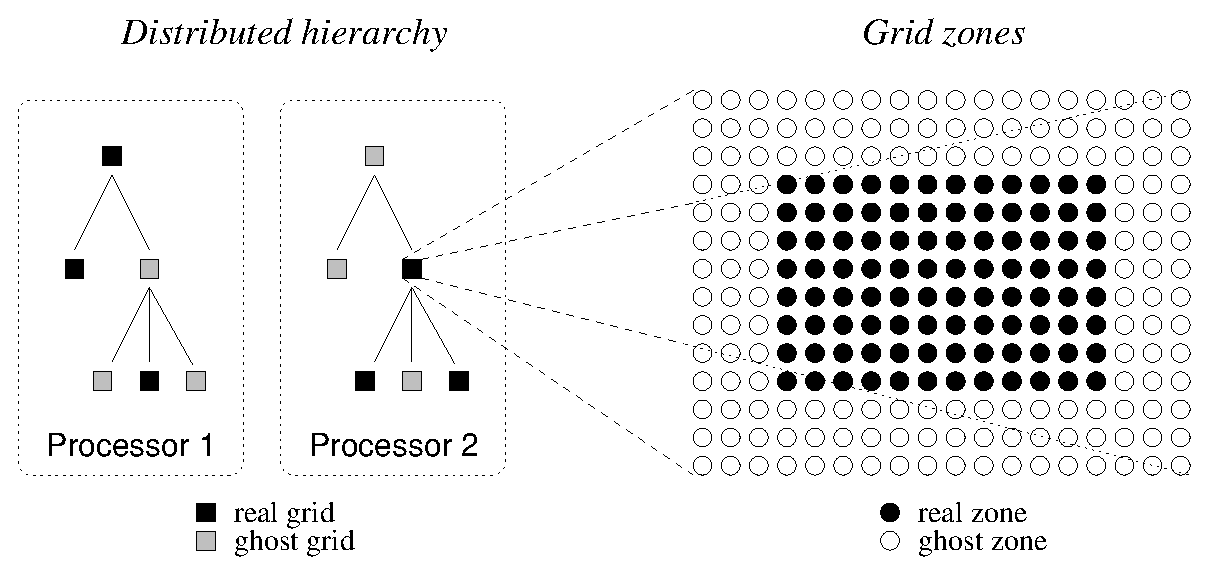
\includegraphics[width=0.4\textwidth]{figures/amr_hierarchy.eps}
\end{center}
\caption{\emph{Left:}  Example of a simple, distributed AMR hierarchy showing real and ghost grids.
\emph{Right:}  Example 2D \enzo\ grid showing real and ghost zones, as 
needed for the PPM hydro stencil. }
\label{fig:amr_hierarchy}
\end{figure}



% ----------------------------------

\subsection{Performance}
\label{sec.performance}

\subsubsection{Performance model \red{(Greg)}}

% Maybe include Greg's text on general scaling arguments

\subsubsection{Performance Measurement \& Instrumentation \red{(Sam)}}

Because of the wide variety of simulations, methods, and uses of Enzo,
it is difficult to define exactly which routines are most costly
during a given simulation.  As such, we have designed a lightweight
registering system that has been implemented for the most commonly
used routines (such as the hydrodynamic and gravity solvers) as well
as refinement level timers that measure the (exclusive) time spent on
each level.  Beyond this minimal set of routines, we have designed a
simple way for the user to modify the source by adding
\texttt{TIMER\_START(``Your Routine Name'')} and
\texttt{TIMER\_END(``Your Routine Name'')}.  These timers are
automatically registered in a
std::map\footnote{http://www.cplusplus.com/reference/map/map/}.  These
timers are created and managed individually on each processor in an
asynchronous fashion.

At each complete EvolveHierarchy (or less often if specified), each timer is
then communicated to the root processor where it calculates the mean, standard
deviation, minimum, and maximum for each of the timers across all processors. 
For level timers, there are also attributes such as the number of cell updates,
the current number of grids, and the average cells/s/MPI process.  This
information is then output to a ``performance.out'' logfile.  This provides a 
simplified interface to the user that can be used to diagnose performance 
issues as well as estimate a given problem type's scalability.  In addition to 
the logfile, we have developed a plotting interface for quickly producing 
figures that process the data from the logfile.  These capabilities are 
described in the online documentation, along with a further discussion of the 
performance measurement implementation.

\subsubsection{Unigrid scaling}

It is advantageous to use \enzo\ in its ``unigrid'' (i.e.,
non-adaptive mesh) mode for a variety of problems, including
non-gravitating turbulence
\citep[e.g.,][]{2002ApJ...569L.127K,Kritsuk04}, the Lyman-alpha forest
\citep{2005MNRAS.361...70J,2009MNRAS.399.1934P}, or feedback of
metal-enriched gas from galaxies into the intergalactic medium
\citep{2004ApJ...601L.115N,2011ApJ...731....6S}.  Achieving good
scaling of the code in unigrid mode is relatively straightforward --
upon initialization, unigrid simulations are decomposed such that each
MPI process has a roughly equal subvolume (and thus number of grid
cells), meaning that work is evenly distributed.  Communication
patterns for both the gravity solve (which uses a fast Fourier
transform) and the fluid solves (which transfer boundary information
between subvolumes) are predictable and straightforward, and
rebuilding of the grid hierarchy does not take place, removing a
substantial global operation and a great deal of communication.

Figure~\ref{fig.uniscale} shows \enzo\ weak scaling results for a
sequence of scaled unigrid Lyman alpha forest calculations. These
calculations include dark matter dynamics, hydrodynamics using the
piecewise parabolic method, six-species non-equilibrium chemistry and
radiative cooling, and a uniform metagalactic ultraviolet background.
In this sequence of test calculations, we perform a weak scaling test
on up to 13,824 MPI tasks on the NICS Kraken XT4 and ORNL Jaguar XT4
supercomputers\footnote{These simulations were performed in 2008,
prior to conversion of both machines to the current-generation
systems}.  In this test, each MPI task was given a $128^3$ root grid
tile (i.e., $128^3$ grid cells containing baryon quantities) and,
initially, approximately $128^3$ dark matter particles.  The number of
grid cells was constant throughout the calculation; the number of dark
matter particles varies as they are moved from subvolume to subvolume
as structure evolves.  The grid resolution was kept at a constant
comoving size of $\simeq 40$~kpc/h, and as the core count was
increased, so was the simulation volume.  On each machine, a compute
node contained a single AMD Opteron quad-core chip (2.1 Ghz on Jaguar;
2.3 Ghz on Kraken) with 2 GB/memory per core (8 GB/total per node).
Both machines used the SeaStar2 interconnect.  In the scaling study,
calculations were run with 1, 2 or 4 MPI tasks per node.  The figure
shows cell updates per second per MPI process; perfect scaling would
be a horizontal line.

As can be seen in Figure~\ref{fig.uniscale}, the unigrid weak scaling
performance of the code is extremely good for this problem, with only
a 20\% decrease in cell updates/second/task as the code is scaled from
8 to 4,096 MPI tasks, and a 40\% decrease in performance overall going
from 8 to 13,824 (or $24^3$) MPI tasks.  We speculate that this
decrease is likely to be partially due to global MPI communications
used to, e.g., calculate the overall timestep of the simulation, and
also likely due to load imbalances due to increasing cosmological
power (and thus an increasingly uneven distribution of dark matter
particles between MPI tasks at late times) as the simulation volume
grows.  We also observe that a systematic difference in speed can be
seen between the two machines, which can be attributed primarily to
the slightly faster CPUs on Kraken (2.3 Ghz, vs. 2.1 Ghz on Jaguar).
The difference in speed when using different numbers of MPI tasks per
node can be attributed primarily due to differences in competing usage
of shared cache on the quad-core chips used on this machine.

Broadly, excellent scaling in \enzo's unigrid mode is seen for a
variety of problems as long as each compute core is given an adequate
amount of work to do.  For cosmological simulations, this seems to be
roughly $128^3$ cells per core.  If fewer cells per core are used, the
CPU is essentially data-starved, and poor scaling is observed due to
computing units being idle while waiting for information to be
communicated from other processes (for, e.g., boundary information or
gravity solves).  Substantially larger cell counts per core would in
principle help scaling by reducing the amount of inter-process
communication needed, but larger cell counts are typically impractical
on most machines due to memory limits.

As a final point, we observe that scaling at larger core counts has
been measured, but only with an experimental hybrid-parallel (MPI +
OpenMP) version of \enzo.  Using this version, scaling comparable to
that shown in Figure~\ref{fig.uniscale} was seen on up to 98,304 cores
on the NICS Kraken XT5 (an upgraded version of the XT4 machine used
for the scaling study shown in the figure), using 2-8 OpenMP threads
per MPI process.  Hybrid parallelism has the potential to
substantially improve scaling by reducing the amount of communication
per grid tile (as described in the previous paragraph); however, the
optimal ratio of OpenMP threads per MPI task seems to vary
substantially between computational platforms and astrophysical
problems/required \enzo\ physics modules, and thus we hesitate to
provide strict guidelines here.

\begin{figure}
\begin{center}
\includegraphics[width=0.4\textwidth]{figures/enzo_unigrid_weak_scaling.eps}
\caption{\enzo\ weak scaling performance for a set of Lyman alpha
forest cosmology simulations with constant comoving spatial resolution
per grid cell, showing cell updates per second per computational core
plotted as a function of the number of root grid tiles of dimension
$128^3$ (R) in each dimension.  The number of MPI tasks is N$ = R^3$,
so R$ = 16$ on this plot corresponds to a $2048^3$ computational mesh
running on 4096 MPI tasks.  This plot goes from R$ = 2$ (8 MPI tasks)
to R$ = 24$ (13,824 MPI tasks) on two supercomputers -- NICS Kraken
and ORNL Jaguar when they were Cray XT4 systems -- and using 1, 2 or 4
MPI processes per node, where each compute node contained a single
quad-core AMD Opteron CPU having a speed of 2.1 GHz on Jaguar and 2.3
GHz on Kraken.}
\label{fig.uniscale}
\end{center}
\end{figure}

\subsubsection{AMR scaling \red{(Greg)}}

% Greg to work on this, scaling data from his runs, or maybe from John Wise

%%% Local Variables: 
%%% mode: latex
%%% TeX-master: "ms"
%%% End: 


%% Section: discussion

%%%%%%%%%%%%%%%%%%%%%%%%%%%%%%%%%%%%%%%%%%%%%%%%%%%%%%%%%%%%%%%%%%%%%%%%%%%%%
\section{Discussion}

\red{
\begin{enumerate}
\item What physics will be put into the code in the next couple of years? (ideal mhd, FLD, ray tracing, more...)
\item What will never be in the code (non-cartesian coordinates, SPH)
\item What are clear areas of improvement?  (gravity solver, maybe more advanced/different hydro methods, parallelization, load balancing)
\item Discuss relative ease of adding new particle types (dust, ``galaxy particles,'' etc.) and some other new packages (cooling).  Other things are harder (MHD, radiation transport).  Outline what's easy and what's hard, in very general terms.
\end{enumerate}
} %end red



%% Section: summary

%%%%%%%%%%%%%%%%%%%%%%%%%%%%%%%%%%%%%%%%%%%%%%%%%%%%%%%%%%%%%%%%%%%%%%%%%%%%%
\section{Summary}

\red{
Recap the physics, performance, how much \enzo\ kicks butt on the various code tests.  This won't be very long.
}


\appendix

%% Appendix: interpolation
%\input{app-interpolation}

%% Appendix:  Data Structures

%%%%%%%%%%%%%%%%%%%%%%%%%%%%%%%%%%%%%%%%%%%%%%%%%%%%%%%%%%%%%%%%%%%%%%%%%%%%%

\section{Data structures}\label{app.datastructure}


The primary data structure in ENZO\ is the {\tt grid}.  
\gtt{It has yet to be determined how much of this
appendix will be in the Method Paper, and how much will be in the
User/Developer Guide.  Green type denotes text that will definitely be
in the User/Developer guide.} \red{Red denotes meta notes-- things to
write, fix, find.}

\subsection{Outline and List of Routines.}
\begin{enumerate}
 \item Creation and Destruction
   \begin{enumerate}
     \item Flow of Rebuild hierarchy: 
       \begin{enumerate}
	 \item delete hierarchy
	 \item build new hierarchy
	 \item scavange from old hierarchy
       \end{enumerate}
     \item Cell Flagging Methods
     \item Grid Fracturing Methods
   \end{enumerate}    
 \item Parallelism
  \begin{enumerate}
    \item Top Grid (block domain decomposition)
    \item Subgrids (memory balance, level by level)(Actually, I think
          its Parent Grid by Parent Grid.)
  \end{enumerate}
 \item Relation to other objects: 
   \begin{enumerate}
     \item Parents (No refinement jump requirements.  Talk about flux
        correction improvement to this effect here?)
     \item Siblings
     \item Children
     \end{enumerate}
 \item Traversing the hierarchy (this might be rolled into the
   previous bullet)
  \begin{enumerate}
    \item Level iterator 
    \item Hierarchy iterator
    \item Grid Array
    \item Chaining Mesh
  \end{enumerate}
  \item Particle treatement
   \begin{enumerate}
     \item Which grid gets the particles
     \item How particles are refined: criteria
     \item How particles are refined: how it fits in with the Grid refinement
   \end{enumerate}
  \item Ghost zones
    \begin{enumerate}
      \item how, when filled
    \end{enumerate}
  \item Timestepping
    \begin{enumerate}
      \item How timestep is determined
      \item Order of level operations: W cycle
    \end{enumerate}
\end{enumerate}
A list of routines to mention: \red{Zeus does this in a big table that
  references code name, what it does, and what equations it
  solves. Might be a useful idea to steal.}
\begin{description}
 \item[\tt{EvolveHierarchy}] Primary timestep control routine. 
 \item[\tt{EvolveLevel}] Primary evolution routine.
 \item[\tt{RebuildHierarchy}] Rebuilds the grid hierarchy
\end{description}

\subsection{Grid Intro}
The life of an \enzo\ simulation centers around the {\tt grid}
object and relationships between individual {\tt grid} instances.  
Grids are independant cartesian patches in space, which contain meta data about
that space (for instance its size, its position in the volume, 
size of the cells in that patch) as well as the data that belongs in
that space (fluid quntities like density and energy, as well as
particle quantites like position and velosity.)

Grids are treated, as individual instances of fluid
dynamics problems, with Dirichlet boundary conditions.  Boundary
conditions, stored in ghost zones, are determined by
one of 3 methods; from user defined exterior conditions like
outflow or reflecting, copied from active zones of 
neighbors, or interpolated from parents.  Grids are group in two
logical structures: a tree like hierarchy that relates parent grids to
children grids; and a level structure that relates grids of the same
refinement.  

\subsection{Creation and Destruction: \tt{RebuildHierarchy}}
Creation and destruction of grids happens in the routine
{\tt RebuildHierarchy}.  
At the end of every timestep, the Hierarchy is rebuilt.
Rebuilding starts at the coarsest level at the point in time (note
that coarser levels may be further ahead in their integration, due to
their larger timestep and the W-cycle)  Beginning with this coarsest level, each
grid on each level is examined for refinement.  Cells are first flagged
based on a variety of criterion, described in section
\ref{sec.flagging}.  The set of flagged cells, stored in the \grid\ memeber
array {\tt FlaggingField}, is then devided into grids as described
in section \ref{app.subgrid_creation}.  Data in these subgrids
is then created by interpolation from the parent using \red{what kind
  of interpolation?}  After this New Subgrid is filled with
interpolated data, the set of Old Subgrids is examined for overlapping
data.  All Old Cells that correspond to New Cells are coppied to the
New Grid.

\subsection{Cell Flagging Methods}\label{sec.flagging}
\enzo\ selects cells to refine based on the physics of the simulation.
Essentially any criterion that can be derived locally from the fluid
data and its derivatives can, in principal, be used to flag the cells
for refinement. Currently, \enzo\ has 8 methods of refinement.
installed, which we will discuss here.  Any or all of these methods may be employed in
any given \enzo\ simulation.  \gtt{Information on how to write your own
refinement criterion can be found Somewhere, to be written}
\begin{description}
  \item[Field Slope] \gtt{grid::FlagCellsToBeRefinedBySlope()} For each
  fluid quantity $u$, a cell $i$ is flagged if 
$$ \frac{u_{i+1}-u_{i-1}}{u_i} > slope $$
  where $slope$ \gtt{\tt MinimumSlopeForRefinement} is
  a  user-defined
  parameter. This is repeated for all
  3 directions. 
  \item[Baryon mass] \gtt{
  grid::FlagCellsToBeRefinedByMass()}  Cells
  are flagged if $$ \rho  V > m_{f} r^{\alpha L} $$ 
  where $V$ is the
  volume of the cell, $r$ is the refinement ratio, $L$ is the grid
  level, $m_{f}$ and ${\alpha}$ are user parameters. \gtt{MinimumMassForRefinement} and 
  \gtt{ MinimumMassForRefinementLevelExponent\[\]}
  \item[Baryon Overdensity] As the name suggests, refines if the
  density is greater than the mean density in the simulation.  In
  practice, this refinement method uses the same machenery as flagging
  by Baryon Mass, with the minimum
  mass for flagging, $m_f$ \gtt{ = MinimumMassForRefinement}, set to the
  input parameter \gtt{MinimumOverDensityForRefinement} times the
  mean density.  \gtt{This is calculted differently for each problem
  generator: consult the source for further documentation}
  \red{This could probably use a word on the effects of
  parameter choices.}
  \item[Shocks] \gtt{
  grid::FlagCellsToBeRefinedByShocks()} \red{This text should be
  updated to reflect Alexei's improvements} A cell $i$ is flagged if it is
  determined to be taking part in a shock.  This is determined if it
  has each of the following:
  \begin{enumerate}
    \item Large relative pressure jump: 
      $$\frac{|p_{i+1} - p_{i-1}| }{min( p_{i+1}, p_{i-1} ) }
      > \gtt{MinimumPressureJumpForRefinement} $$
     \item compression: $$ u_{i+1} < u_{i-1} $$
    \item More thermal energy than Kinetic: $$ \frac{
    \frac{p_i}{\gamma -1} }{ \frac{1}{2}\rho v^2 } > \gtt{
    MinimumEnergyRatioForRefinement } $$ \red{why?}
  \end{enumerate}  
  \item[Particle Mass] Using the Cloud In Cell interpolation method,
  described  \red{elsewhere?}, particle data is interpolated to the
  Eulerian grid cell centers.  A cell is flagged if the resulting mass field passes
  the ``RefineByMass'' test, described above.
  \item[Jeans Length] If a gravitationally collapsing simulation is
  under-resolved, artificial fragmentation can occur.  It was
  descoverd experimentally by \red{Truelove; get citation}
  that sufficient resolution was achieved if the Jeans Length is
  resolved by at least 4 cells.  This is determined if 
  $$ dx^2 >
  \frac{\alpha}{N_{cells} \gtt{= RefineByJeansLengthSafetyFactor}}\frac{T_{i,j,k}}{\rho_{i,j,k}} $$
  
  and $\alpha = \frac{\pi k_b }{G m_{proton} }*
  \frac{LengthUnits^2}{DensityUnits}$

  \red{dude, double check this.}
  \item[Cooling Time]  \red{Finish this.}

  \item[Shear] For highly turbulent flows, it may be useful to resolve
  shear layers.  This is done whenever
  $$\frac{\partial v_x}{\partial y}^2 + \frac{\partial v_x}{\partial z}^2 
  > \eta \gtt{= MinimumShearForRefinement}
  $$
  In practice, $$\frac{\partial v_x}{\partial y} = 
  u_{j+1}-u_{j-1}$$
  The same is done for $v_y$ and $v_z$
  
\end{description}

\subsection{Grid Fracturing}\label{app.subgrid_creation}
Once the cells in a given grid are flagged for refinement, they're
broken into a set of subgrids by an iterative process.  This process
first draws a minimally enclosing box around the set of flagging
cells, and generates a {\tt ProtoSubgrid}.  A {\tt ProtoSubgrid} is
essentially just the spatial extent and flagging field that will
define the spatial extent of the future \grid.  Each {\tt
  ProtoSubgrid} is then examined for efficiency (the ratio of flagged cells to
total), total size (for cache optimization) and minimum side
length (to avoid a flock of one zone grids).  {\tt ProtoSubgrid} that are too
large or not efficient enough are broken into smaller grids, by a
process to be described shortly, new minimally enclosing boxes are
drawn around each of the two remaining flagging fields, and new {\tt
  ProtoSubgrid}s are created.  This process is then repeated until
all {\tt ProtoSubgrid}s are both small enough and efficient enough.
It should be noted that \enzo\ does not glue grids back together-- the
Minimum Side Length is enforced by not examining the other two
conditions if the {\tt ProtoSubgrid} is too small.  

Maximum size, minimum side length,  and minimum efficiency are
controlled by the parameters {\tt MaximumSubgridSize}, {\tt MinimumSubgridEdge} and {\tt
  MinimumEfficiency}, respectivly. Typical maximum sizes are 10000 zones, minimum
side lengths are typically 5 zones, and minimum efficiencies are  0.2.
Choice of these parameters, especially maximum size, are
based on the architecture of the computer in question.  
Machines with larger cache sizes will benifit from larger values for
{\tt MaximumSubgridSize}, as communication and memory overhead from
ghost zones will be reduced; machines with smaller cache sizes benifit
from lower values, in that the computational time is reduced for a
grid that can fit entirely into cache.  

A {\tt ProtoSubgrid} that fails either the efficency or size
requirement is then broken into smaller {\tt ProtoSubgrid}s by a
method that tries to preserve physically continuous structures onto
individual grids.  The process examines the 1d Signature of the Flagging
field, which is the projection of the Flagging Field along two of the
coordinate axes.  First, each of the 3 signature fields is examined
for zeros.  Zeros in the signature field indicates disjoint
structures, so the {\tt ProtoSubgrid} is first cut into two smaller
ones along that line.  If no such cuts can be made, zero crossings of
the second derivative in the signature are then looked for.  Zero
crossings in the second derivative indicates edges of structures.  If
more than one exists, the 'strongest crossing,' that is the largest
jump, is selected for the cut.  If no such zero crossings can be
found, the {\tt ProtoSubgrid} is then cut evenly along the longest
axis.  See figure \ref{fig.signature} for a schematic of this process.

\begin{figure}
\begin{center}
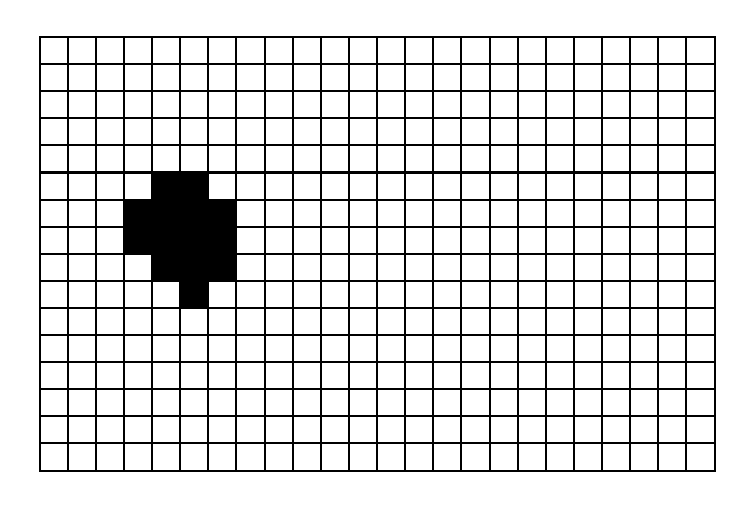
\includegraphics[width=0.4\textwidth]{figures/SignatureSchematic.eps}
\end{center}
\caption{
Schematic of Flagging Field and Signature.  Cuts will be made along
some line I'll draw.  The figure will be improved in the future.
}
\label{fig.signature}
\end{figure}







%% Appendix:  I/O

\section{I/O}

\red{It's not clear whether this section needs to exist.  Comments welcome.}

\red{Talk about standard serial IO, parallel IO (root grid + 
nested grid + particles), packed IO.  Why does this make a difference?}



%% Appendix:  Zeus hydro
%
\section{The ZEUS hydro method}
\red{ 
\begin{enumerate}
 \item Compare ZEUS-MP 2.0 (Hayes et al) paper  to \enzo.  Only put discrepancies here, cite specific sections of that paper.
 \item Addition of cosmology:  difference equations updated.
\end{enumerate}
}%end red


%% Appendix:  PPM hydro
%
\section{The PPM hydro method}\label{app.ppm}
\red{
\begin{enumerate}
  \item Cite \citet{1995CoPhC..89..149B} for Lagrangian Remap version
  \item State that Lagrangian Remap it doesn't really work and nobody uses it (why is that?)
  \item Brief overview of PPM: 
  \begin{enumerate}
    \item Parabolic reconstruction
    \item Order Lowering near shocks
    \item Characteristic tracing for Left and Right states
    \item I don't remember if we use a contact steepener:  If yes,
    describe.  If no, say so.
  \end{enumerate}
  \item Repeat bits of \citet{1984JCoPh..54..174C} that have been altered
        for cosmology 
  \item I think C\&W 1984 discuss gravity: double check we do the
  same.  If not, comment.
  \item Discus TwoShock solver, 
    \begin{enumerate} 
       \item Short method review, I think Woodward 1986.
       \item Discuss Rarefaction updates 
       \item Discuss alterations for Expansion
       \item Discuss alterations for Gravity (if not in Woodward 1986)
    \end{enumerate}
\end{enumerate}
}%end red


%% Appendix:  gravity solver
%
\section{Gravity solver}

\red{This needs to be fleshed out a lot - basically we want to emphasize how we solve the
root grid (mention parallelization strategy for FFT), how the potentials calculated are 
interpolated to subgrids for the multigrid solution on the subgrids, and how particles are 
actually moved.
}

\red{**********  Which version of the gravity solver will we be using for the public release?  
The new Dan Reynolds mulgrid-everywhere solver, or the one that's currently in the public
release?  Alter paper and other documentation accordingly.}

With and without cosmology - how does this affect what is solved/how it's solved?
Why do we do $\rho-\bar{\rho}$ instead of just $\rho$?  What is the finite difference
equation that you actually solve in the end?

How are particles interpolated to grids, and accelerations from grid
to particles? 

\subsection{multigrid}
This is for James.

\subsection{leapfrog integrator}
Talk about how particles' accelerations are calculated, etc.



%% Appendix:  

\section{Primordial chemistry and cooling}\label{app:chemistry}

\red{This currently just describes the rates solver without any radiation
backgrounds.  Improve this to include terms for radiation backgrounds (including
photoionizing and lyman-werner) and, if necessary, explain how these
terms fit in there.}

The primordial chemistry network implemented in \enzo\ is discussed in 
Section~\ref{sec.ov.chem} and also in
much more detail by~\citet{abel97} and~\citet{anninos97}.  
These papers describe the chemistry and cooling behavior of low-density primordial gas
($n \simeq 10^4$ and below), as well as
the steps that are necessary to obtain fast and accurate numerical solutions of the 
nonequilibrium chemical reaction rate network.  This network is extended by
~\citet{ABN02} to include the 3-body molecular hydrogen creation process, 
which becomes important at higher densities, and extends the validity of the reaction
network several more orders of magnitude in density, essentially until the gas becomes
optically thick to cooling by $H_2$ line emission. 
For the sake of completeness, and because the properties the primordial gas are so 
crucial to the results that are discussed in this work, we describe the chemistry 
network in this appendix.

Tables~\ref{table.collisional} and~\ref{table.radiative} summarize the collisional
and radiative processes solved in the \enzo\ nonequilibrium chemistry routines.  
\citet{abel97} show that accurate results can be obtained if several unnecessary
reactions are eliminated and the reaction network is reduced to the following:


\begin{eqnarray}
\frac{d \nd{H} }{dt}    &=& \k{2} \nd{\mHp} \nd{e} - \k{1} \nd{H} \nd{e} + 2 \k{31} \nd{\mHH}  \\
\frac{d\nd{\mHp}}{dt}  &=& \k{1} \nd{H}   \nd{e} - \k{2} \nd{\mHp}  \nd{e}      \\
\frac{d\nd{He} }{dt}  &=& \k{4} \nd{\mHep}\nd{e} - \k{3} \nd{He}   \nd{e}       \\
\frac{d\nd{\mHep}}{dt} &=& \k{3} \nd{He} \nd{e} + \k{6} \nd{\mHepp}\nd{e} -
                       \k{4} \nd{\mHep}\nd{e}                           \\
\frac{d\nd{\mHepp}}{dt}&=& \k{5} \nd{\mHep}\nd{e} - \k{6} \nd{\mHepp} \nd{e}    \\
\frac{d\nd{\mHH} }{dt}  &=& \k{8} \nd{\mHm} \nd{H} + \k{22} \nd{H}^3 - \nd{\mHH}   \left( 
        \k{31} + \k{11} \nd{\mHp} + \k{12} \nd{e} \right), 
\end{eqnarray}

where the number density of \Hm is given by the equilibrium condition

\begin{eqnarray}
\nd{\mHm} = {\k{7} \nd{H} \nd{e}  \over \k{8} \nd{H}  + 
 \k{16} \nd{\mHp} + \k{14} \nd{e}}.
\end{eqnarray}

The \Hm number density can be calculated in equilibrium because the timescale at which the
reactions controlling its number density occur are much shorter than the rest of the 
reactions in this system.  The rate coefficients used in the equations above are defined as follows:

\begin{eqnarray}       
 k_1 & = & \exp[-32.71396786 + 13.536556  \ln(T) - 5.73932875   \ln(T)^2 \nonumber \\ 
     &   & + 1.56315498  \ln(T)^3  - 0.2877056 \ln(T)^4 + 3.48255977\times 10^{-2} \times\ln(T)^5  \nonumber \\
     &   & - 2.63197617\times 10^{-3}\times\ln(T)^6 +  1.11954395\times 10^{-4}   \ln(T)^7 \nonumber \\
     &   & -  2.03914985 \times 10^{-6}   \ln(T)^8]~{\rm cm^3~s^{-1}}
\end{eqnarray}

\begin{eqnarray}
 k_2 &=& \exp[-28.6130338 - 0.72411256  \ln(T) - 2.02604473\times10^{-2}  \ln(T)^2  \nonumber \\
     & &   - 2.38086188\times10^{-3}  \ln(T)^3 - 3.21260521\times10^{-4}  \ln(T)^4  \nonumber \\
     & &   - 1.42150291\times10^{-5}  \ln(T)^5 + 4.98910892  \times10^{-6} \ln(T)^6  \nonumber \\
     & &   + 5.75561414 \times10^{-7}   \ln(T)^7 - 1.85676704 \times10^{-8}   \ln(T)^8 \nonumber \\
     & &   - 3.07113524 \times10^{-9}   \ln(T)^9]~{\rm cm^3~s^{-1}}
\end{eqnarray}

\begin{eqnarray}
 k_3 &=& \exp[ (-44.09864886 + 23.91596563   \ln(T) -  10.7532302   \ln(T)^2 \nonumber \\
     & &   + 3.05803875   \ln(T)^3 - 0.56851189   \ln(T)^4 + 6.79539123 \times 10^{-2}  \ln(T)^5  \nonumber \\
     & &   - 5.00905610 \times 10^{-3}   \ln(T)^6 + 2.06723616 \times 10^{-4} \ln(T)^7 \nonumber \\
     & &   - 3.64916141 \times 10^{-6}   \ln(T)^8)~{\rm cm^3~s^{-1}}
\end{eqnarray}

\begin{eqnarray}
k_{4r} & = & 3.925 \times 10^{-13}T^{-0.6353}~{\rm cm^3 s^{-1} } \\
k_{4d} &=& 1.544 \times 10^{-9} T^{-\frac{3}{2}} 
     \exp\left( - \frac{48.596~eV}{T} \right) \times \nonumber \\
   & &     \left[0.3 + \exp\left(\frac{8.10~eV}{T}\right)\right]~{\rm cm^3~s^{-1}}
\end{eqnarray}

\begin{eqnarray}
k_5 & = & \exp[-68.71040990 + 43.93347633   \ln(T) - 18.4806699   \ln(T)^2 \nonumber \\
    & &   + 4.70162649   \ln(T)^3 - 0.76924663   \ln(T)^4 + 8.113042 \times 10^{-2} \ln(T)^5 \nonumber \\
    & &   - 5.32402063 \times 10^{-3}  \ln(T)^6 +  1.97570531\times 10^{-4}  \ln(T)^7 \nonumber \\
    & &   - 3.16558106 \times 10^{-6}  \ln(T)^8]~{\rm cm^3~s^{-1}}
\end{eqnarray}

\begin{eqnarray}
k_6 = 3.36 \times 10^{-10} T^{-\frac{1}{2}}
\left(\frac{T}{1000\K}\right)^{-0.2}
\left(1+\left(\frac{T}{10^6\K}\right)^{0.7}\right)^{-1}~{\rm cm^3~s^{-1}}
\end{eqnarray}

$k_7$ for T $\leq 6000$~K:

\begin{eqnarray} 
k_7 & = & 1.429 \times 10^{-18} T^{0.7620} T^{0.1523 \log_{10}(T)}  T^{-3.274 \times 10^{-2} \log_{10}^2(T)}~{\rm cm^3~s^{-1}} \nonumber \\
\end{eqnarray}

$k_7$ for T $ > 6000$~K:

\begin{eqnarray}  
k_7 & = & 3.802 \times 10^{-17} T^{0.1998 \log_{10}(T)}  \nonumber \\
    &   & {\rm dex} \left( { 4.0415 \times 10^{-5} \log_{10}^6(T)  - 5.447 \times 10^{-3} \log_{10}^4(T)}~{\rm cm^3~s^{-1}}\right)
\end{eqnarray}

\begin{eqnarray}
T&>&0.1~{\rm eV}:\ k_8 = \exp[-20.06913897 +0.22898   \ln(T) +  3.5998377  \nonumber \\
 &&       \times 10^{-2}   \ln(T)^2 - 4.55512 \times 10^{-3}  \ln(T)^3- 3.10511544\times 10^{-4}   \ln(T)^4   \nonumber \\
 &&       + 1.0732940 \times 10^{-4}  \ln(T)^5 -  8.36671960 \times 10^{-6}   \ln(T)^6 + 2.23830623 \nonumber \\
  &&      \times 10^{-7}   \ln(T)^7]~{\rm cm^3~s^{-1}} . \\
T &<& 0.1~{\rm eV}:  k_8  =  1.428 \times 10^{-9}~{\rm cm^3~s^{-1}}
\end{eqnarray}

\begin{eqnarray}
\ln(k_{11}) & = &   -24.24914687 + 3.40082444  \ln(T) - 3.89800396  \ln(T)^2  \nonumber \\
             & &       +  2.04558782  \ln(T)^3 -  0.541618285  \ln(T)^4   + 8.41077503 \times 10^{-2}  \ln(T)^5 \nonumber \\
             & &       - 7.87902615 \times 10^{-3} \ln(T)^6 \nonumber + 4.13839842 \times 10^{-4} \ln(T)^7 \nonumber \\
             & &       - 9.36345888\times 10^{-6}  \ln(T)^8 {\rm cm^3 s^{-1}}
\end{eqnarray}


\begin{eqnarray}
\ \ k_{12} = 5.6 \times 10^{-11} T^\frac{1}{2} \exp(-\frac{102,124 K}{T}) {\rm cm^3 s^{-1}}
\end{eqnarray}


\begin{eqnarray}
k_{14}&=& \exp[-18.01849334 + 2.3608522   \ln(T) - 0.28274430   \ln(T)^2   \nonumber \\
      & &    + 1.62331664 \times 10^{-2}  \ln(T)^3 - 3.36501203 \times 10^{-2} \ln(T)^4   \nonumber \\
      & &    + 1.17832978 \times 10^{-2}   \ln(T)^5 - 1.65619470 \times 10^{-3} \ln(T)^6   \nonumber \\
      & &    + 1.06827520 \times 10^{-4}   \ln(T)^7 - 2.63128581 \times 10^{-6} \ln(T)^8) {\rm cm^3 s^{-1}}
\end{eqnarray}


\begin{eqnarray}\ \ k_{16} = 7 \times 10^{-8} \left( \frac{T}{100{\rm
        K}} \right)^{-\frac{1}{2}} {\rm cm^3 s^{-1}} 
\end{eqnarray}

$k_{22}$ For T $< 300$~K:

\begin{eqnarray}
k_{22} & = & 1.3 \times 10^{-32} (T / 300 {\rm K} )^{-0.38} {\rm cm^6 s^{-1}}
\end{eqnarray}

$k_{22}$ for T $\geq 300$~K:

\begin{eqnarray}
k_{22} & = & 1.3 \times 10^{-32} (T / 300 {\rm K} )^{-1} {\rm cm^6 s^{-1}}
\end{eqnarray}

The photodissociation of molecular hydrogen by Lyman-Werner radiation is controlled by the $k_{31}$ parameter: 

\begin{eqnarray}
k_{31} & = & 1.13 \times 10^8~{\rm F_{LW} }~|t|
\end{eqnarray}

where $|t| \equiv ( 4 \pi G \Omega_m \rho_c (1+z_i)^3)^{-1/2}$
and has units of seconds, and F$_{LW}$ is the Lyman-Werner background flux in 
units of~erg~s$^{-1}$~cm$^{-2}$~Hz$^{-1}$.


% this is the end!


\bibliographystyle{apj}
\bibliography{apj-jour,ms}  % looks in ms.bib for bibliography info

\end{document}  


